\section*{CHAPTER 2. THEORETICAL BACKGROUND}
\addcontentsline{toc}{section}{CHAPTER 2. THEORETICAL BACKGROUND}

% =========================================================
% Numbering for Chapter 2
% =========================================================
\setcounter{section}{2}
\setcounter{subsection}{0}
\setcounter{subsubsection}{0}
\setcounter{figure}{0}
\setcounter{table}{0}
\setcounter{equation}{0}

\renewcommand{\thefigure}{2.\arabic{figure}}
\renewcommand{\thetable}{2.\arabic{table}}
\renewcommand{\theequation}{2.\arabic{equation}}
\renewcommand{\theHfigure}{2.\arabic{figure}}
\renewcommand{\theHtable}{2.\arabic{table}}
\renewcommand{\theHequation}{2.\arabic{equation}}

% =========================================================
% Chapter Introduction
% =========================================================
This chapter presents the theoretical foundations required for the study of OTFS and OTFS-IM systems. Fundamental concepts related to wireless communication channels, multipath propagation, Doppler effects, OFDM transmission, delay-Doppler signal representation, and index modulation techniques are reviewed~\cite{Hong2019OTFSTutorial,Basar2016IndexMod5G,Wen2017OFDMIM}. These concepts provide the necessary background for the development and analysis of the proposed systems in the subsequent chapters.


% =========================================================
% Chapter Sections
% =========================================================
\subsection{Wireless Communication Channels}

Wireless communication channels provide the medium through which information is transmitted between communicating devices. Due to the random nature of the propagation environment, wireless signals are affected by various phenomena that influence transmission quality and system performance. Therefore, understanding the characteristics, impairments, and classification of wireless channels is essential for the design and analysis of modern communication systems.

\subsubsection{Wireless Channel Characteristics}

A wireless communication channel represents the physical medium through which electromagnetic waves propagate from a transmitter to a receiver. Unlike wired channels, where the transmission medium is fixed and relatively predictable, wireless channels are inherently dynamic and strongly influenced by the surrounding environment. Buildings, vehicles, terrain, and moving objects may alter the propagation path of transmitted signals, resulting in significant variations in the received waveform.

In communication theory, a wireless channel is commonly modeled as a linear system that modifies the transmitted signal during propagation. The received signal can generally be expressed as

\begin{equation}
y(t)=h(t)\ast x(t)+n(t)
\end{equation}

where $x(t)$ is the transmitted signal, $y(t)$ is the received signal, $h(t)$ denotes the channel impulse response, $\ast$ represents the convolution operation, and $n(t)$ denotes additive noise.

The channel impulse response contains information regarding the propagation environment and determines how the transmitted signal is transformed before reaching the receiver. Variations in the channel response arise from factors such as propagation distance, obstacles, mobility, and environmental conditions.

\begin{figure}[H]
    \centering

    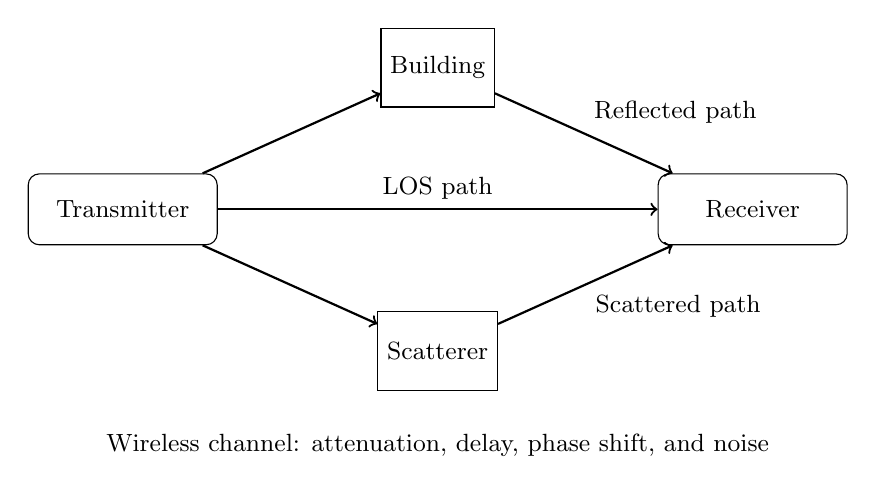
\begin{tikzpicture}[
        every node/.style={font=\small},
        block/.style={
            draw,
            rounded corners,
            minimum width=2.4cm,
            minimum height=0.9cm,
            align=center
        },
        obj/.style={
            draw,
            minimum width=1.2cm,
            minimum height=1.0cm,
            align=center
        },
        arrow/.style={->, thick}
    ]

    % Transmitter and receiver
    \node[block] (tx) at (0,0) {Transmitter};
    \node[block] (rx) at (8,0) {Receiver};

    % Objects
    \node[obj] (building) at (4,1.8) {Building};
    \node[obj] (scatterer) at (4,-1.8) {Scatterer};

    % Direct path
    \draw[arrow] (tx) -- node[above] {LOS path} (rx);

    % Reflected path
    \draw[arrow] (tx) -- (building);
    \draw[arrow] (building) -- node[above right] {Reflected path} (rx);

    % Scattered path
    \draw[arrow] (tx) -- (scatterer);
    \draw[arrow] (scatterer) -- node[below right] {Scattered path} (rx);

    % Channel label
    \node[align=center] at (4,-3.0)
    {Wireless channel: attenuation, delay, phase shift, and noise};

    \end{tikzpicture}

    \caption{General representation of a wireless communication channel.}
    \label{fig:wireless_channel_model}
\end{figure}

Figure~\ref{fig:wireless_channel_model} illustrates a typical wireless propagation scenario. Instead of following a single direct path, the transmitted signal may arrive at the receiver through multiple propagation paths generated by reflection, diffraction, and scattering mechanisms.

The unique characteristics of wireless channels distinguish them from wired transmission media. Signal attenuation increases with propagation distance, multiple signal replicas may be received due to multipath propagation, and mobility introduces time-varying channel behavior. These characteristics collectively create significant challenges for reliable wireless communication.

\subsubsection{Channel Impairments}

During propagation, wireless signals are subjected to various impairments that degrade transmission quality and limit communication performance. These impairments originate from the physical characteristics of the propagation environment as well as from practical limitations of communication hardware. Understanding their effects is essential for the design of reliable wireless transmission systems.

One of the most fundamental impairments is path loss, which refers to the gradual reduction in signal power as the propagation distance increases. In practical environments, obstacles such as buildings, vegetation, and terrain irregularities introduce additional attenuation, commonly known as shadowing. These effects reduce the received signal strength and may significantly limit communication coverage.

Another important impairment is multipath fading. Due to reflections, diffraction, and scattering, multiple copies of the transmitted signal arrive at the receiver through different propagation paths. Since these signal components experience different delays and phases, constructive and destructive interference may occur, leading to fluctuations in the received signal amplitude and phase.

Wireless communication systems are also affected by Doppler effects caused by relative motion between the transmitter, receiver, or surrounding scatterers. Doppler shifts introduce frequency offsets and time variations into the channel response, which become increasingly significant in high-mobility scenarios such as vehicular communications, high-speed railways, and unmanned aerial vehicle networks.

In addition, all practical receivers are affected by thermal noise generated by electronic components. This disturbance is commonly modeled as Additive White Gaussian Noise (AWGN) and represents a fundamental source of performance degradation in wireless communication systems.

\begin{figure}[H]
    \centering

    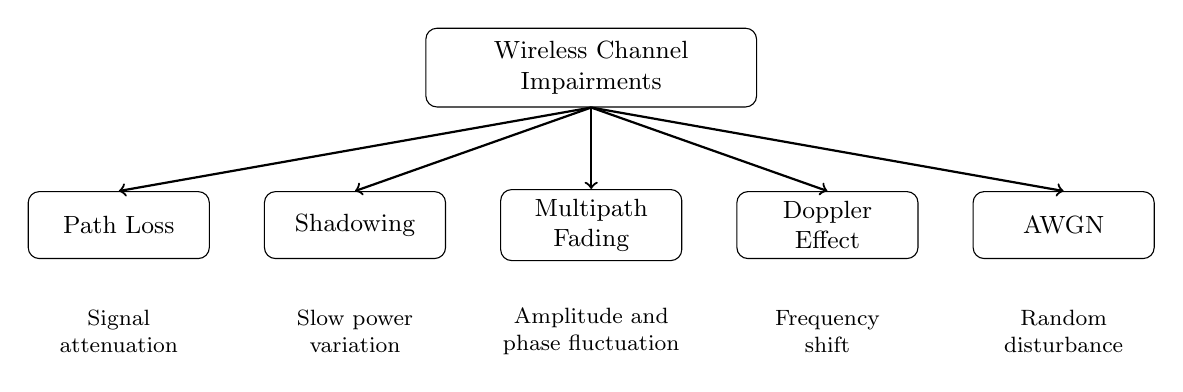
\begin{tikzpicture}[
        every node/.style={font=\small},
        main/.style={
            draw,
            rounded corners,
            minimum width=4.2cm,
            minimum height=1.0cm,
            align=center
        },
        item/.style={
            draw,
            rounded corners,
            minimum width=2.3cm,
            minimum height=0.85cm,
            align=center
        },
        desc/.style={
            align=center,
            font=\footnotesize
        },
        arrow/.style={->, thick}
    ]

    % Main node
    \node[main] (channel) at (0,0) {Wireless Channel\\Impairments};

    % Impairment nodes - increased spacing
    \node[item] (pathloss)  at (-6.0,-2.0) {Path Loss};
    \node[item] (shadowing) at (-3.0,-2.0) {Shadowing};
    \node[item] (multipath) at (0,-2.0) {Multipath\\Fading};
    \node[item] (doppler)   at (3.0,-2.0) {Doppler\\Effect};
    \node[item] (noise)     at (6.0,-2.0) {AWGN};

    % Arrows
    \draw[arrow] (channel.south) -- (pathloss.north);
    \draw[arrow] (channel.south) -- (shadowing.north);
    \draw[arrow] (channel.south) -- (multipath.north);
    \draw[arrow] (channel.south) -- (doppler.north);
    \draw[arrow] (channel.south) -- (noise.north);

    % Descriptions
    \node[desc] at (-6.0,-3.35) {Signal\\attenuation};
    \node[desc] at (-3.0,-3.35) {Slow power\\variation};
    \node[desc] at (0,-3.35) {Amplitude and\\phase fluctuation};
    \node[desc] at (3.0,-3.35) {Frequency\\shift};
    \node[desc] at (6.0,-3.35) {Random\\disturbance};

    \end{tikzpicture}

    \caption{Major impairments affecting wireless communication channels.}
    \label{fig:channel_impairments}
\end{figure}

The major impairments encountered in wireless communication channels and their corresponding effects are summarized in Table~\ref{tab:channel_impairments}.

\begin{table}[H]
\centering
\caption{Common wireless channel impairments and their effects.}
\label{tab:channel_impairments}

\begin{tabular}{|p{3cm}|p{4cm}|p{6cm}|}
\hline
\textbf{Impairment} &
\textbf{Primary Cause} &
\textbf{Effect on System Performance} \\
\hline

Path Loss &
Propagation distance &
Reduction of received signal power \\
\hline

Shadowing &
Obstacles and terrain &
Slow fluctuations in received signal strength \\
\hline

Multipath Fading &
Multiple propagation paths &
Amplitude and phase variations, signal distortion \\
\hline

Doppler Effect &
Relative motion &
Frequency shifts and channel time variations \\
\hline

AWGN &
Thermal noise &
Detection errors and performance degradation \\
\hline

\end{tabular}

\end{table}

The combined effects of path loss, fading, Doppler shifts, and noise represent the primary challenges faced by modern wireless communication systems. These impairments directly influence the design of modulation schemes, channel estimation algorithms, equalization techniques, and receiver architectures. Consequently, accurate channel modeling is a crucial step in the development and evaluation of advanced communication technologies.


\subsubsection{Channel Classification}

Wireless communication channels can be classified according to different characteristics of the propagation environment. Such classifications provide useful insight into channel behavior and help communication engineers select appropriate transmission and receiver techniques for specific operating conditions.

Based on frequency selectivity, wireless channels are generally categorized as flat-fading channels or frequency-selective channels. In a flat-fading channel, all frequency components of the transmitted signal experience approximately the same channel gain and phase shift. Conversely, a frequency-selective channel affects different frequency components differently, resulting in signal distortion and potential inter-symbol interference.

From a temporal perspective, channels may be classified as time-invariant or time-varying. A time-invariant channel remains relatively stable during the transmission interval, whereas a time-varying channel exhibits continuous fluctuations due to user mobility and changes in the propagation environment.

Wireless channels can also be categorized according to propagation conditions. Line-of-Sight (LOS) channels contain a direct propagation path between the transmitter and receiver, while Non-Line-of-Sight (NLOS) channels rely mainly on reflected, diffracted, and scattered signal components.

Table~\ref{tab:channel_classification} summarizes several common criteria used for wireless channel classification.

\begin{table}[H]
\centering
\caption{Classification of wireless communication channels.}
\label{tab:channel_classification}

\begin{tabular}{|p{4cm}|p{4cm}|p{4cm}|}
\hline
\textbf{Classification Criterion} &
\textbf{Category 1} &
\textbf{Category 2} \\
\hline

Frequency Selectivity &
Flat Fading &
Frequency Selective \\
\hline

Time Variation &
Time Invariant &
Time Varying \\
\hline

Propagation Condition &
LOS &
NLOS \\
\hline

Mobility Scenario &
Low Mobility &
High Mobility \\
\hline

\end{tabular}

\end{table}

\begin{figure}[H]
    \centering

    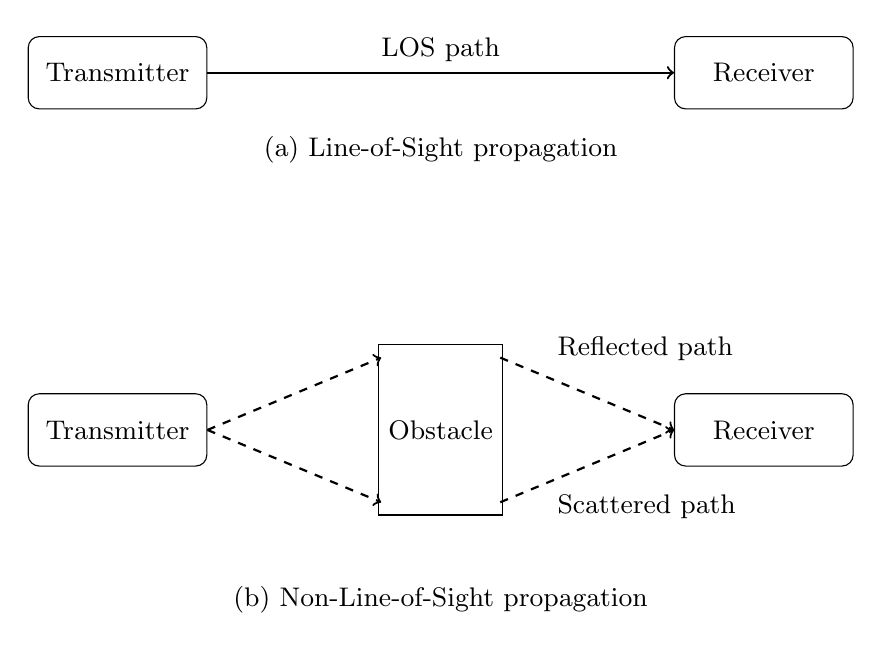
\begin{tikzpicture}[
        scale=1.08,
        transform shape,
        every node/.style={font=\small},
        device/.style={
            draw,
            rounded corners,
            minimum width=2.1cm,
            minimum height=0.85cm,
            align=center
        },
        obstacle/.style={
            draw,
            minimum width=1.45cm,
            minimum height=2.0cm,
            align=center
        },
        arrow/.style={->, thick},
        dashedarrow/.style={->, thick, dashed}
    ]

    % =========================
    % LOS scenario
    % =========================
    \node[device] (tx1) at (0,2.2) {Transmitter};
    \node[device] (rx1) at (7.6,2.2) {Receiver};

    \draw[arrow] (tx1.east) -- node[above] {LOS path} (rx1.west);

    \node[align=center] at (3.8,1.3) {(a) Line-of-Sight propagation};

    % =========================
    % NLOS scenario
    % =========================
    \node[device] (tx2) at (0,-2.0) {Transmitter};
    \node[obstacle] (obs) at (3.8,-2.0) {Obstacle};
    \node[device] (rx2) at (7.6,-2.0) {Receiver};

    % Points near obstacle edges (shorter dashed arrows)
    \coordinate (topL) at (3.1,-1.15);
    \coordinate (topR) at (4.5,-1.15);
    \coordinate (botL) at (3.1,-2.85);
    \coordinate (botR) at (4.5,-2.85);

    % Dashed paths
    \draw[dashedarrow] (tx2.east) -- (topL);
    \draw[dashedarrow] (topR) -- (rx2.west);

    \draw[dashedarrow] (tx2.east) -- (botL);
    \draw[dashedarrow] (botR) -- (rx2.west);

    % Labels moved away from paths
    \node[anchor=west] at (5.05,-1.05) {Reflected path};
    \node[anchor=west] at (5.05,-2.9) {Scattered path};

    \node[align=center] at (3.8,-4.0) {(b) Non-Line-of-Sight propagation};

    \end{tikzpicture}

    \caption{Illustration of LOS and NLOS propagation scenarios.}
    \label{fig:los_nlos}
\end{figure}

Among the various channel categories, high-mobility wireless channels represent one of the most challenging communication environments. In such scenarios, the channel often exhibits both frequency selectivity due to multipath propagation and time selectivity due to Doppler effects. These characteristics lead to the so-called doubly selective channel, which plays a central role in the development of advanced waveform technologies such as OTFS. The propagation mechanisms responsible for these effects are discussed in the following section.


% ~6 pages
\subsection{Multipath Propagation and Doppler Effects}

The performance of wireless communication systems is strongly affected by the physical propagation environment. In practice, wireless signals rarely propagate through a single ideal path. Instead, they are influenced by surrounding objects, user mobility, and the relative motion between transmitters, receivers, and scatterers. Among these effects, multipath propagation and Doppler effects are particularly important because they determine how the wireless channel varies over time and frequency.

In high-mobility scenarios such as vehicular communications, high-speed railways, unmanned aerial vehicles, and low-earth-orbit satellite links, these effects become more severe. Multipath propagation causes the transmitted signal to arrive at the receiver through multiple paths with different delays, while Doppler effects introduce frequency shifts and time variation. These two phenomena provide the basis for understanding doubly selective channels, which are one of the main motivations for advanced waveform designs such as OTFS.

\begin{figure}[H]
    \centering
    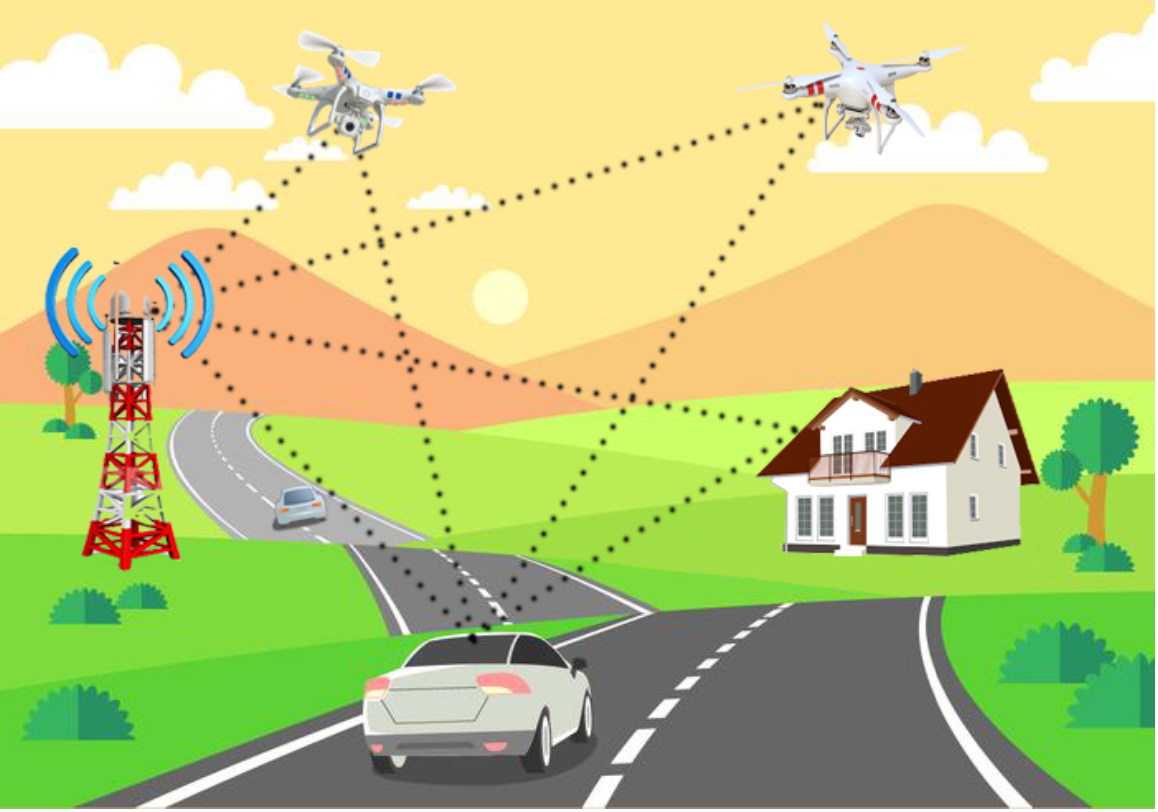
\includegraphics[width=0.82\textwidth]{Images/Chapter2/high_mobility_multipath.png}
    \caption[High-mobility wireless communication scenario with multiple propagation paths.]{High-mobility wireless communication scenario with multiple propagation paths~\protect\cite{Hong2019OTFSTutorial}.}
    \label{fig:high_mobility_multipath}
\end{figure}

Figure~\ref{fig:high_mobility_multipath} illustrates a high-mobility wireless communication scenario in which several terminals and reflecting objects coexist. The transmitted signal may reach the receiver through direct, reflected, diffracted, and scattered paths. Such a propagation environment leads naturally to both delay dispersion and Doppler dispersion.

\subsubsection{Multipath Propagation}

Multipath propagation occurs when transmitted electromagnetic waves reach the receiver through more than one propagation path. These paths may be created by reflection from buildings, diffraction around obstacles, and scattering from irregular objects such as trees, vehicles, and terrain. As a result, the receiver observes several replicas of the transmitted signal rather than a single clean copy.

Each propagation path is generally associated with a different path length. Therefore, the corresponding received signal component has its own delay, amplitude attenuation, and phase shift. The received waveform is formed by the superposition of all these components. Depending on their relative phases, the multipath components may combine constructively or destructively, causing fluctuations in the received signal strength.

A simple multipath channel can be represented as

\begin{equation}
h(t,\tau)=\sum_{i=1}^{P}h_i(t)\delta(\tau-\tau_i),
\end{equation}

where \(P\) is the number of propagation paths, \(h_i(t)\) is the complex channel gain of the \(i\)-th path, and \(\tau_i\) is the propagation delay of that path. This equation only states that the channel is composed of several delayed copies of the transmitted signal.

Figure~\ref{fig:high_mobility_multipath} illustrates the basic idea of multipath propagation. In addition to a possible direct path between the transmitter and receiver, the signal may also arrive through reflected or scattered paths. These additional paths usually travel longer distances and therefore arrive later than the direct component.

Multipath propagation is important because it directly affects the received signal quality. If the delayed components arrive within a short time interval, they may simply cause fading. However, if the delay differences are comparable to the symbol duration, different symbols may overlap at the receiver. This effect is known as inter-symbol interference (ISI).

Although multipath propagation is often considered a source of distortion, it may also provide diversity. Since different propagation paths carry different versions of the transmitted signal, a properly designed receiver can exploit these components to improve reliability. Modern wireless systems use equalization, coding, diversity combining, and multicarrier modulation to reduce the negative effects of multipath and, when possible, benefit from the available path diversity.

In the context of this thesis, multipath propagation is important because it leads to delay spread and frequency selectivity. These concepts are discussed in the next subsection.

\subsubsection{Delay Spread and Frequency Selectivity}

Delay spread is a direct consequence of multipath propagation. Since different propagation paths have different lengths, their corresponding signal components arrive at the receiver at different times. The difference between the earliest and latest significant arriving components is commonly referred to as delay spread.

The propagation delay of a signal path is proportional to the path length and can be expressed as

\begin{equation}
\tau=\frac{d}{c},
\end{equation}

where \(d\) is the propagation distance and \(c\) is the speed of light.

\begin{figure}[H]
    \centering
    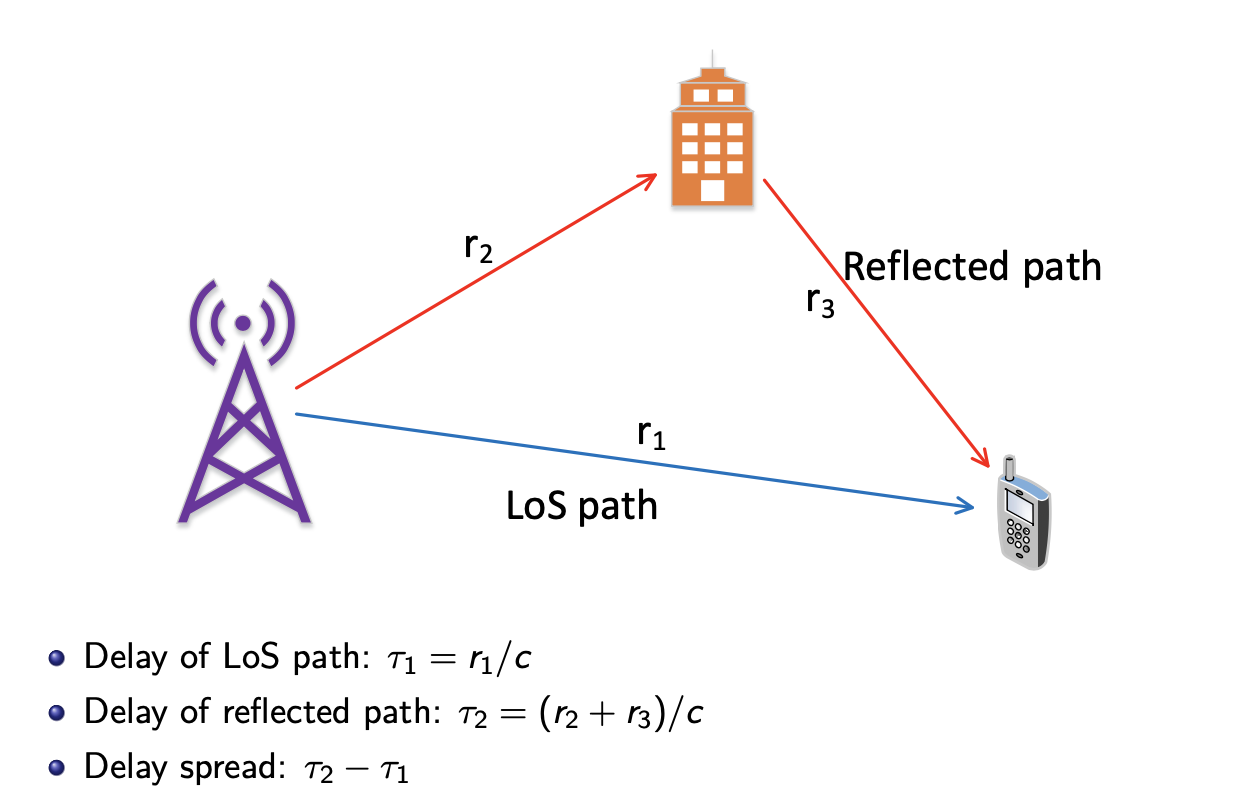
\includegraphics[width=0.82\textwidth]{Images/Chapter2/delay_spread.png}
    \caption[Illustration of delay spread caused by LoS and reflected propagation paths.]{Illustration of delay spread caused by LoS and reflected propagation paths~\protect\cite{Hong2019OTFSTutorial}.}
    \label{fig:delay_spread}
\end{figure}

Figure~\ref{fig:delay_spread} shows a simple example of delay spread. The direct Line-of-Sight (LoS) path travels a distance \(r_1\), while the reflected path travels through two segments with distances \(r_2\) and \(r_3\). Therefore, the corresponding delays can be written as

\begin{equation}
\tau_1=\frac{r_1}{c},
\qquad
\tau_2=\frac{r_2+r_3}{c}.
\end{equation}

The delay spread in this simple case is the difference between these two delays. A larger delay spread means that the received signal components are more spread out in time.

Delay spread has an important effect on the frequency-domain behavior of the channel. When a channel introduces significant delay dispersion, different frequency components of the transmitted signal may experience different attenuation and phase rotation. In this case, the channel is called frequency selective.

If the signal bandwidth is small compared with the frequency range over which the channel response is approximately constant, the channel behaves like a flat-fading channel. In a flat-fading channel, all frequency components of the signal are affected in nearly the same way. Conversely, when the signal bandwidth is large, different frequency components may experience different channel gains. The channel then becomes frequency selective.

Frequency selectivity is a major challenge for broadband communication systems. It can distort the transmitted waveform and create ISI. This is one of the main reasons why OFDM has been widely used in modern wireless systems: OFDM divides a wideband frequency-selective channel into many narrowband subchannels, making equalization much simpler.

Table~\ref{tab:delay_spread_effects} summarizes the relationship between multipath propagation, delay spread, and frequency selectivity.

\begin{table}[H]
\centering
\caption{Effects of multipath propagation and delay spread.}
\label{tab:delay_spread_effects}

\begin{tabular}{|p{4cm}|p{4cm}|p{5cm}|}
\hline
\textbf{Cause} &
\textbf{Channel Effect} &
\textbf{Main Consequence} \\
\hline

Multiple propagation paths &
Different arrival times &
Delay spread \\
\hline

Large delay spread &
Different response across frequency &
Frequency-selective fading \\
\hline

Frequency-selective fading &
Waveform distortion &
Inter-symbol interference \\
\hline

Narrowband transmission &
Nearly constant channel response &
Flat fading \\
\hline

Wideband transmission &
Different gains over the signal bandwidth &
Frequency selectivity \\
\hline

\end{tabular}

\end{table}

For the purpose of this thesis, it is sufficient to understand that delay spread describes how much the signal is dispersed in time, while frequency selectivity describes how differently the channel affects different frequency components. These concepts are essential for understanding why OFDM is effective against multipath, but they do not fully explain high-mobility channels. To characterize mobility, Doppler effects must also be considered.

\subsubsection{Doppler Shift and Doppler Spread}

Doppler effects occur when there is relative motion between the transmitter, receiver, or surrounding scatterers. In wireless communications, such motion causes a shift in the observed carrier frequency. This frequency shift is known as the Doppler shift.

For a propagation path arriving at an angle \(\theta\) relative to the direction of motion, the Doppler shift can be expressed as

\begin{equation}
f_D=\frac{f_c v}{c}\cos\theta,
\end{equation}

where \(f_c\) is the carrier frequency, \(v\) is the relative velocity, \(c\) is the speed of light, and \(\theta\) is the angle between the direction of motion and the direction of wave propagation.

\begin{figure}[H]
    \centering
    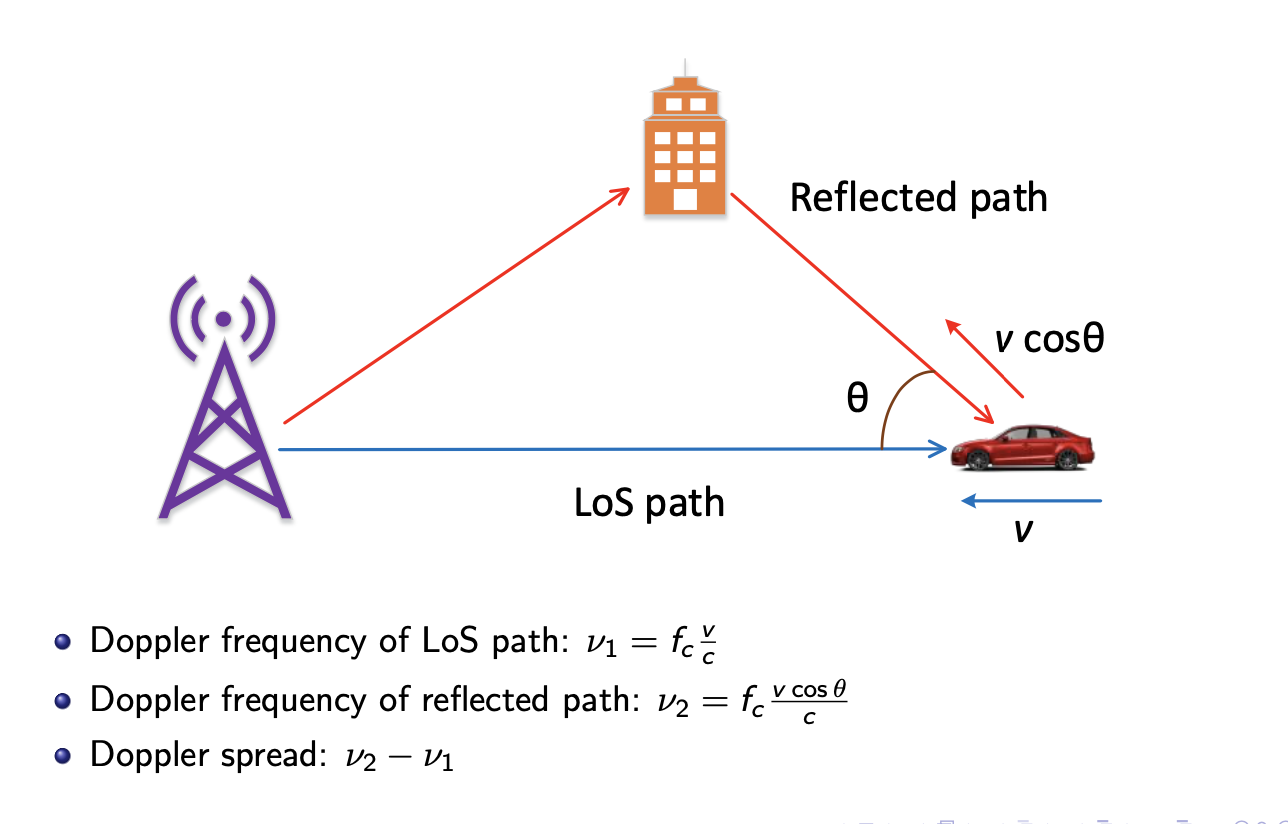
\includegraphics[width=0.82\textwidth]{Images/Chapter2/doppler_spread.png}
    \caption[Illustration of Doppler shift and Doppler spread in a wireless channel.]{Illustration of Doppler shift and Doppler spread in a wireless channel~\protect\cite{Hong2019OTFSTutorial}.}
    \label{fig:doppler_spread}
\end{figure}

Figure~\ref{fig:doppler_spread} illustrates the Doppler effect in a mobile wireless channel. For the LoS path, the motion is assumed to be aligned with the propagation direction, so the Doppler shift can be written as \(f_D=f_c v/c\). For the reflected path, only the velocity component along the propagation direction contributes to the Doppler shift, resulting in \(f_D=f_c v\cos\theta/c\). Since different propagation paths may arrive from different directions, they experience different Doppler shifts.

When multiple propagation paths are present, the received signal contains a range of Doppler shifts rather than a single frequency offset. This range is called Doppler spread. A small Doppler spread means that the channel varies slowly with time, while a large Doppler spread indicates a rapidly time-varying channel.

Doppler spread describes how much the received signal is spread in frequency due to motion. A small Doppler spread means that the channel varies slowly with time. A large Doppler spread means that the channel changes rapidly. Therefore, Doppler spread is closely related to time selectivity.

In low-mobility systems, the wireless channel may remain nearly constant over several symbol intervals. In this case, conventional channel estimation and equalization methods are usually effective. However, in high-mobility environments, the channel may change significantly during a transmission frame or even within one OFDM symbol. This rapid variation makes detection more difficult and may lead to serious performance degradation.

The Doppler effect is particularly important for OFDM systems. OFDM relies on the orthogonality among subcarriers. When the channel varies rapidly due to large Doppler spread, this orthogonality may be destroyed. As a result, energy from one subcarrier leaks into neighboring subcarriers, producing inter-carrier interference (ICI).

Table~\ref{tab:doppler_effects} summarizes the main effects of Doppler shift and Doppler spread.

\begin{table}[H]
\centering
\caption{Effects of Doppler shift and Doppler spread.}
\label{tab:doppler_effects}

\begin{tabular}{|p{4cm}|p{4cm}|p{5cm}|}
\hline
\textbf{Cause} &
\textbf{Channel Effect} &
\textbf{Main Consequence} \\
\hline

Relative motion &
Frequency shift of each path &
Doppler shift \\
\hline

Multiple moving paths &
Range of Doppler shifts &
Doppler spread \\
\hline

Large Doppler spread &
Rapid channel variation &
Time selectivity \\
\hline

Time-selective channel &
Loss of subcarrier orthogonality &
Inter-carrier interference \\
\hline

High mobility &
Fast time-varying channel response &
Difficult channel estimation and equalization \\
\hline

\end{tabular}

\end{table}

In summary, delay spread is mainly associated with multipath propagation, while Doppler spread is mainly associated with mobility. Delay spread causes frequency selectivity, whereas Doppler spread causes time selectivity. Both effects appear simultaneously in many practical high-mobility systems.

\subsubsection{Doubly Selective Channels}

A wireless channel is called doubly selective when it is both frequency selective and time selective. Frequency selectivity is caused by delay spread, while time selectivity is caused by Doppler spread. Therefore, doubly selective channels appear when multipath propagation and mobility occur simultaneously.

Doubly selective channels are common in high-mobility wireless communication scenarios. Examples include high-speed railways, vehicular networks, unmanned aerial vehicles, and low-earth-orbit satellite communications. In these scenarios, the transmitted signal experiences multiple propagation paths and rapid channel variation at the same time.

\begin{figure}[H]
    \centering

    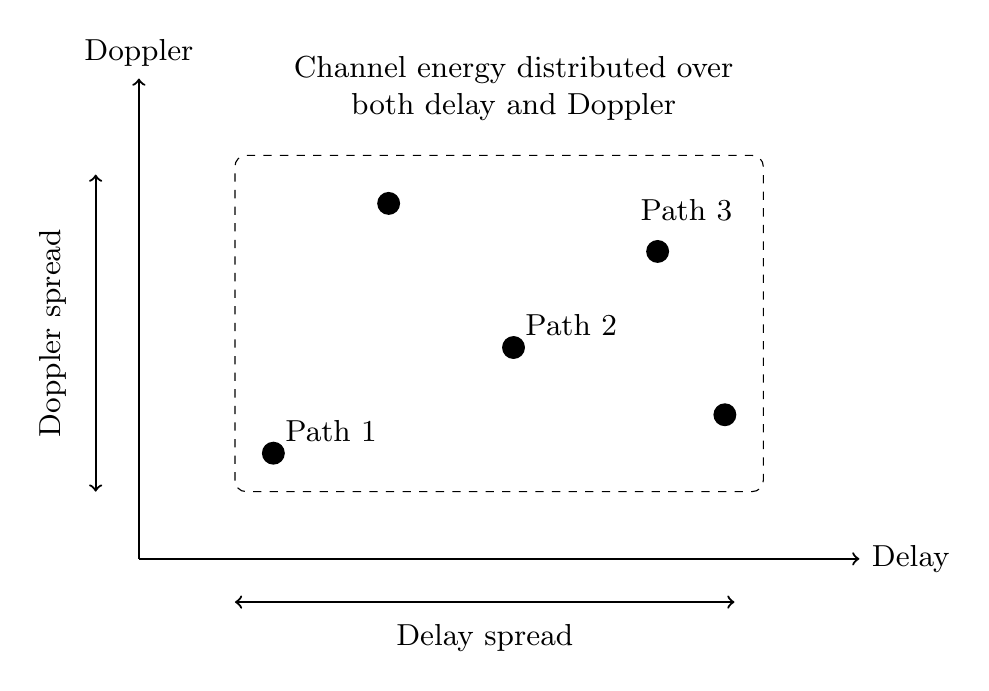
\begin{tikzpicture}[
        scale=1.22,
        transform shape,
        every node/.style={font=\small},
        axis/.style={->, thick},
        pathpoint/.style={circle, fill=black, inner sep=2.4pt},
        spread/.style={draw, dashed, rounded corners}
    ]

    % Axes
    \draw[axis] (0,0) -- (7.5,0) node[right] {Delay};
    \draw[axis] (0,0) -- (0,5.0) node[above] {Doppler};

    % Dashed area showing channel support
    \draw[spread] (1.0,0.7) rectangle (6.5,4.2);

    % Title inside the figure, moved away from y-axis label
    \node[align=center] at (3.9,4.9)
    {Channel energy distributed over\\both delay and Doppler};

    % Delay and Doppler spread indication
    \draw[<->, thick] (1.0,-0.45) -- (6.2,-0.45);
    \node at (3.6,-0.82) {Delay spread};

    \draw[<->, thick] (-0.45,0.7) -- (-0.45,4.0);
    \node[rotate=90] at (-0.9,2.35) {Doppler spread};

    % Path points
    \node[pathpoint] at (1.4,1.1) {};
    \node[pathpoint] at (2.6,3.7) {};
    \node[pathpoint] at (3.9,2.2) {};
    \node[pathpoint] at (5.4,3.2) {};
    \node[pathpoint] at (6.1,1.5) {};

    % Labels
    \node[above right] at (1.4,1.1) {Path 1};
    \node[above right] at (3.9,2.2) {Path 2};
    \node[above right] at (5.1,3.4) {Path 3};

    \end{tikzpicture}

    \caption{Conceptual illustration of a doubly selective channel with both delay and Doppler dispersion.}
    \label{fig:doubly_selective_channel}
\end{figure}

Figure~\ref{fig:doubly_selective_channel} conceptually illustrates a doubly selective channel. The delay dimension represents multipath-induced time dispersion, while the Doppler dimension represents mobility-induced frequency dispersion. Instead of being concentrated around a single propagation component, the channel energy is distributed across both delay and Doppler dimensions.

From a communication system perspective, doubly selective channels are difficult because they introduce both ISI and ICI. Delay spread may cause symbols to overlap in time, leading to ISI. Doppler spread may destroy subcarrier orthogonality, leading to ICI. When both effects are present, receiver design becomes significantly more challenging.

\begin{table}[H]
\centering
\caption{Relationship between propagation effects and channel selectivity.}
\label{tab:channel_selectivity}

\begin{tabular}{|p{4cm}|p{4cm}|p{5cm}|}
\hline
\textbf{Propagation Effect} &
\textbf{Channel Characteristic} &
\textbf{Resulting Impairment} \\
\hline

Delay spread &
Frequency selectivity &
Inter-symbol interference \\
\hline

Doppler spread &
Time selectivity &
Inter-carrier interference \\
\hline

Delay spread and Doppler spread &
Doubly selective channel &
ISI and ICI simultaneously \\
\hline

\end{tabular}

\end{table}

The concept of a doubly selective channel is central to the motivation of OTFS. OFDM can effectively deal with frequency-selective fading when the channel is approximately constant over one OFDM symbol. However, in high-Doppler environments, the channel changes rapidly and the simple diagonal subcarrier model of OFDM is no longer valid. This leads to significant performance degradation.

For this reason, waveform designs for future high-mobility communications must handle both delay and Doppler effects. OTFS addresses this problem by representing information symbols in the delay-Doppler domain, where the wireless channel can often be described more compactly in terms of physical propagation paths. Before discussing OTFS in detail, the next section reviews OFDM, which remains the dominant waveform in current wireless communication systems and provides a useful reference point for understanding the need for OTFS.


% ~8 pages
\subsection{Orthogonal Frequency Division Multiplexing}

Orthogonal Frequency Division Multiplexing (OFDM) has become the dominant waveform technology in modern wireless communication systems due to its high spectral efficiency and implementation simplicity. OFDM has been adopted in numerous communication standards, including LTE, 5G NR, Wi-Fi, and digital broadcasting systems. Before discussing the limitations of OFDM in high-mobility environments and the motivation for OTFS modulation, it is necessary to understand its fundamental operating principles.

\subsubsection{Principles of OFDM}

Orthogonal Frequency Division Multiplexing (OFDM) is a multicarrier transmission technique that divides a high-rate data stream into multiple parallel low-rate data streams. These streams are transmitted simultaneously over a set of orthogonal subcarriers, thereby reducing the symbol rate associated with each subcarrier and improving robustness against frequency-selective fading.

Unlike conventional Frequency Division Multiplexing (FDM), where adjacent subcarriers must be separated by guard bands to prevent interference, OFDM exploits the orthogonality between subcarriers to allow significant spectral overlap. As a result, OFDM achieves high spectral efficiency while maintaining the ability to separate individual subcarriers at the receiver.

The baseband OFDM signal can be expressed as

\begin{equation}
s(t)=\sum_{k=0}^{N-1} X_k e^{j2\pi k\Delta f t},
\quad 0 \le t < T
\end{equation}

where \(X_k\) denotes the complex symbol transmitted on the \(k\)-th subcarrier, \(N\) is the total number of subcarriers, and \(\Delta f\) represents the subcarrier spacing.

The key feature of OFDM is the orthogonality among subcarriers. Two subcarriers are orthogonal when

\begin{equation}
\int_{0}^{T}
e^{j2\pi n\Delta f t}
e^{-j2\pi m\Delta f t}
dt
=
0,
\quad n \neq m
\end{equation}

which is satisfied when the subcarrier spacing is chosen as

\begin{equation}
\Delta f = \frac{1}{T}
\end{equation}

where \(T\) denotes the OFDM symbol duration.

\begin{figure}[H]
    \centering
    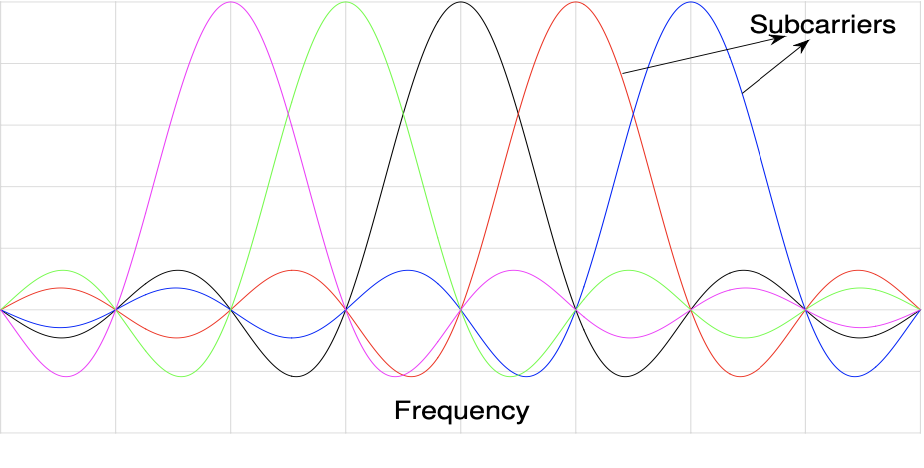
\includegraphics[width=1\textwidth]{Images/Chapter2/ofdmsubcarrier.png}
    \caption[Orthogonality among OFDM subcarriers.]{Orthogonality among OFDM subcarriers~\protect\cite{ScienceDirectICI}.}
    \label{fig:ofdm_orthogonality}
\end{figure}

As illustrated in Fig.~\ref{fig:ofdm_orthogonality}, the spectrum of each subcarrier exhibits a sinc-shaped response. Although adjacent subcarriers overlap significantly in the frequency domain, the peak of one subcarrier coincides with the null points of all other subcarriers. Consequently, mutual interference is avoided and the transmitted symbols can be recovered independently.

A major advantage of OFDM is its efficient implementation using the Inverse Fast Fourier Transform (IFFT) and Fast Fourier Transform (FFT). At the transmitter, information symbols are mapped onto frequency-domain subcarriers and transformed into the time domain using an IFFT operation. At the receiver, an FFT operation is applied to recover the transmitted symbols from the received waveform.

\begin{figure}[H]
    \centering
    \resizebox{0.95\textwidth}{!}{
    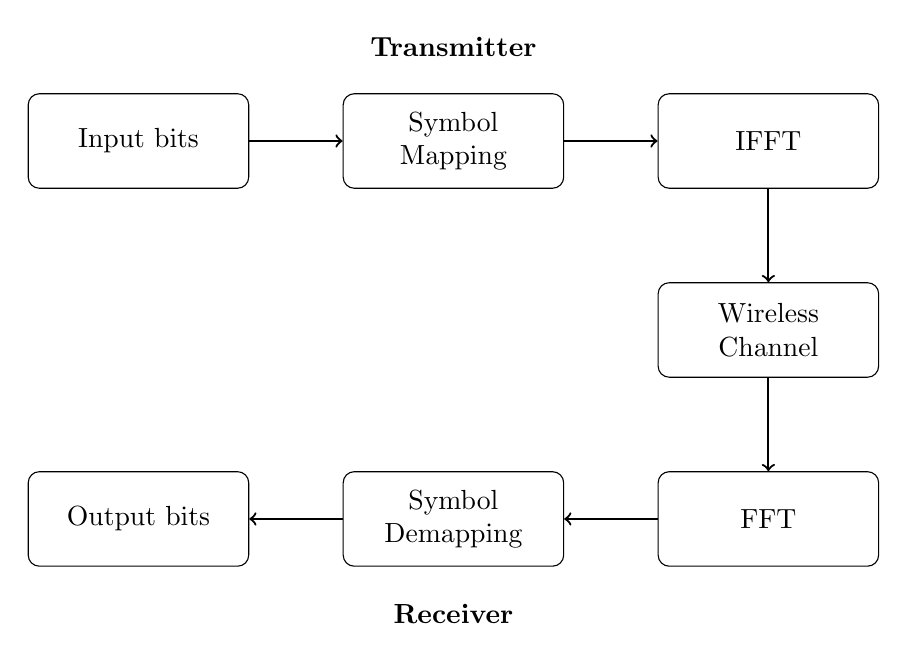
\begin{tikzpicture}[
        block/.style={
            draw,
            rounded corners,
            minimum width=2.8cm,
            minimum height=1.2cm,
            align=center,
            font=\normalsize
        },
        arrow/.style={->, thick}
    ]

    % =========================
    % Transmitter
    % =========================
    \node[block] (in)   at (0,2.4) {Input bits};
    \node[block] (map)  at (4.0,2.4) {Symbol\\Mapping};
    \node[block] (ifft) at (8.0,2.4) {IFFT};

    \draw[arrow] (in) -- (map);
    \draw[arrow] (map) -- (ifft);

    \node[font=\bfseries] at (4.0,3.6) {Transmitter};

    % =========================
    % Channel
    % =========================
    \node[block] (channel) at (8.0,0) {Wireless\\Channel};
    \draw[arrow] (ifft) -- (channel);

    % =========================
    % Receiver
    % =========================
    \node[block] (fft)   at (8.0,-2.4) {FFT};
    \node[block] (demap) at (4.0,-2.4) {Symbol\\Demapping};
    \node[block] (out)   at (0,-2.4) {Output bits};

    \draw[arrow] (channel) -- (fft);
    \draw[arrow] (fft) -- (demap);
    \draw[arrow] (demap) -- (out);

    \node[font=\bfseries] at (4.0,-3.6) {Receiver};

    \end{tikzpicture}
    }
    \caption{Basic principle of OFDM transmission using IFFT and FFT operations.}
    \label{fig:ofdm_basic_principle}
\end{figure}

By converting a broadband frequency-selective channel into multiple narrowband subchannels, OFDM significantly simplifies receiver design and equalization. This property has contributed to its widespread adoption in modern wireless communication systems. However, despite these advantages, OFDM experiences considerable performance degradation in rapidly time-varying channels, particularly under high Doppler conditions. These limitations are discussed in the following subsections.


\subsubsection{OFDM Transceiver Structure}

The practical implementation of OFDM systems is based on digital signal processing techniques that efficiently generate and recover orthogonal subcarriers using IFFT and FFT operations. Instead of using a large number of separate oscillators and modulators for different subcarriers, OFDM generates all subcarriers jointly through an inverse Fourier transform. This significantly reduces implementation complexity while maintaining high spectral efficiency.

A typical OFDM transceiver consists of a transmitter, a wireless propagation channel, and a receiver. At the transmitter, the input binary data stream is first converted into parallel data streams. These bits are then mapped into complex modulation symbols using modulation schemes such as BPSK, QPSK, or QAM. The resulting symbols are assigned to different frequency-domain subcarriers.

To generate the time-domain OFDM waveform, an \(N\)-point Inverse Fast Fourier Transform (IFFT) is applied to the frequency-domain symbols. The IFFT converts the parallel subcarrier symbols into a discrete-time OFDM signal while preserving the orthogonality among subcarriers. The transmitted OFDM symbol can be expressed as

\begin{equation}
x[n]
=
\frac{1}{\sqrt{N}}
\sum_{k=0}^{N-1}
X[k]
e^{j\frac{2\pi kn}{N}},
\quad n=0,1,\ldots,N-1,
\end{equation}

where \(X[k]\) denotes the modulation symbol transmitted on the \(k\)-th subcarrier and \(N\) represents the total number of subcarriers.

In practical OFDM systems, a cyclic prefix (CP) is often appended to each OFDM symbol before transmission. The CP is formed by copying the last portion of the OFDM symbol and inserting it at the beginning of the symbol interval. This operation helps mitigate inter-symbol interference (ISI) caused by multipath propagation and allows the linear convolution of the channel to be treated approximately as circular convolution. As a result, frequency-domain equalization at the receiver becomes much simpler.

\begin{figure}[H]
    \centering
    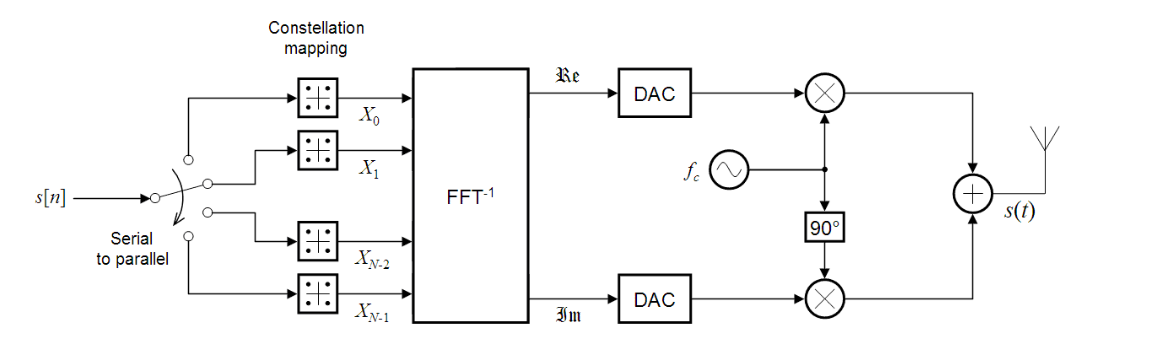
\includegraphics[width=0.92\textwidth]{Images/Chapter2/ofdmtx.png}
    \caption[OFDM transmitter structure.]{OFDM transmitter structure~\protect\cite{Hong2019OTFSTutorial}.}
    \label{fig:ofdm_tx}
\end{figure}

\begin{figure}[H]
    \centering
    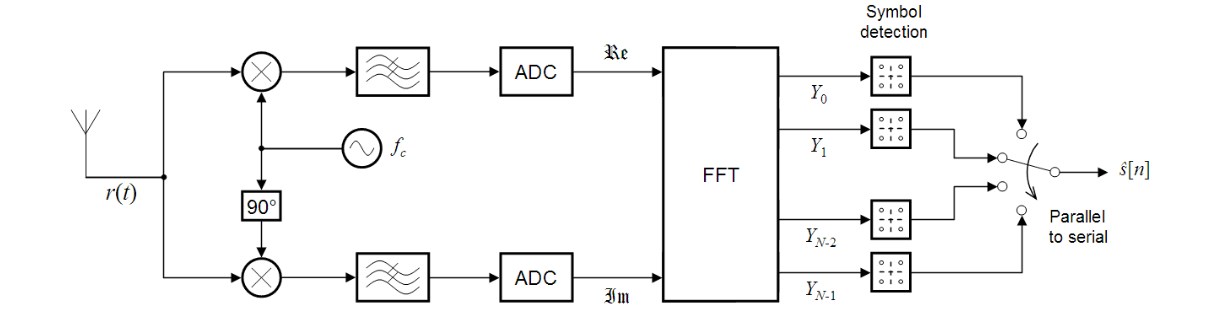
\includegraphics[width=0.92\textwidth]{Images/Chapter2/ofdmrx.png}
    \caption[OFDM receiver structure.]{OFDM receiver structure~\protect\cite{Hong2019OTFSTutorial}.}
    \label{fig:ofdm_rx}
\end{figure}



As illustrated in Fig.~\ref{fig:ofdm_tx}, the transmitter performs serial-to-parallel conversion, constellation mapping, IFFT processing, digital-to-analog conversion, and carrier modulation before radiating the signal through the antenna. The IFFT block is the key baseband processing stage because it converts frequency-domain subcarrier symbols into a time-domain waveform suitable for transmission.

After propagating through the wireless channel, the received signal is affected by multipath fading, Doppler shifts, and additive noise. At the receiver, the signal is first downconverted from the carrier frequency, filtered, and converted back into digital samples. The FFT operation is then applied to transform the received time-domain signal back into the frequency domain. Symbol detection and parallel-to-serial conversion are finally performed to recover the estimated transmitted bit sequence.

Under the assumption that the channel remains approximately constant during one OFDM symbol interval and that the CP is sufficiently long, the received symbol on the \(k\)-th subcarrier can be represented as

\begin{equation}
Y[k]
=
H[k]X[k]
+
W[k],
\end{equation}

where \(Y[k]\) is the received symbol on the \(k\)-th subcarrier, \(H[k]\) denotes the channel frequency response, \(X[k]\) is the transmitted symbol, and \(W[k]\) represents the noise component.

Because each OFDM subcarrier experiences an approximately flat channel response, equalization can be performed independently for each subcarrier. This one-tap frequency-domain equalization greatly reduces receiver complexity compared with single-carrier systems operating over frequency-selective channels.

The use of FFT-based processing and simple per-subcarrier equalization is one of the main reasons for the widespread adoption of OFDM in modern wireless communication systems. However, these advantages rely on the assumption that the channel is nearly time-invariant within each OFDM symbol. In high-mobility environments, Doppler spread causes rapid channel variation and may destroy the orthogonality among subcarriers, resulting in inter-carrier interference and degraded system performance.


\subsubsection{Advantages of OFDM}

OFDM has been widely adopted in modern wireless communication systems because it provides an efficient solution for transmission over frequency-selective fading channels. By dividing a wideband channel into a large number of narrowband orthogonal subchannels, OFDM simplifies the equalization problem and enables reliable high-data-rate transmission.

One of the most important advantages of OFDM is its robustness against multipath propagation. In a single-carrier system, multipath delay spread may cause severe inter-symbol interference because delayed replicas of previous symbols overlap with the current symbol. In OFDM, the symbol duration on each subcarrier is increased by transmitting data in parallel over many subcarriers. As a result, the relative impact of delay spread is reduced.

Another major advantage is the use of the cyclic prefix. When the cyclic prefix length is longer than the maximum delay spread of the channel, the linear convolution between the transmitted signal and the multipath channel can be transformed into circular convolution. This allows the frequency-selective channel to be represented as a set of parallel flat-fading subchannels after the FFT operation at the receiver.

Under ideal synchronization and sufficiently slow channel variation, the received signal on each subcarrier follows the one-tap input-output relation introduced in the previous subsection. Since the transmitted symbols are separated in the frequency domain, each subcarrier can be equalized independently using a one-tap equalizer.

The estimated transmitted symbol can therefore be obtained as

\begin{equation}
\hat{X}[k]=\frac{Y[k]}{H[k]},
\end{equation}

where \(H[k]\) is the channel frequency response on the \(k\)-th subcarrier.

This one-tap frequency-domain equalization is one of the key reasons for the practical success of OFDM. Compared with time-domain equalization in wideband single-carrier systems, OFDM significantly reduces receiver complexity.

\begin{figure}[H]
    \centering
    \resizebox{0.95\textwidth}{!}{
    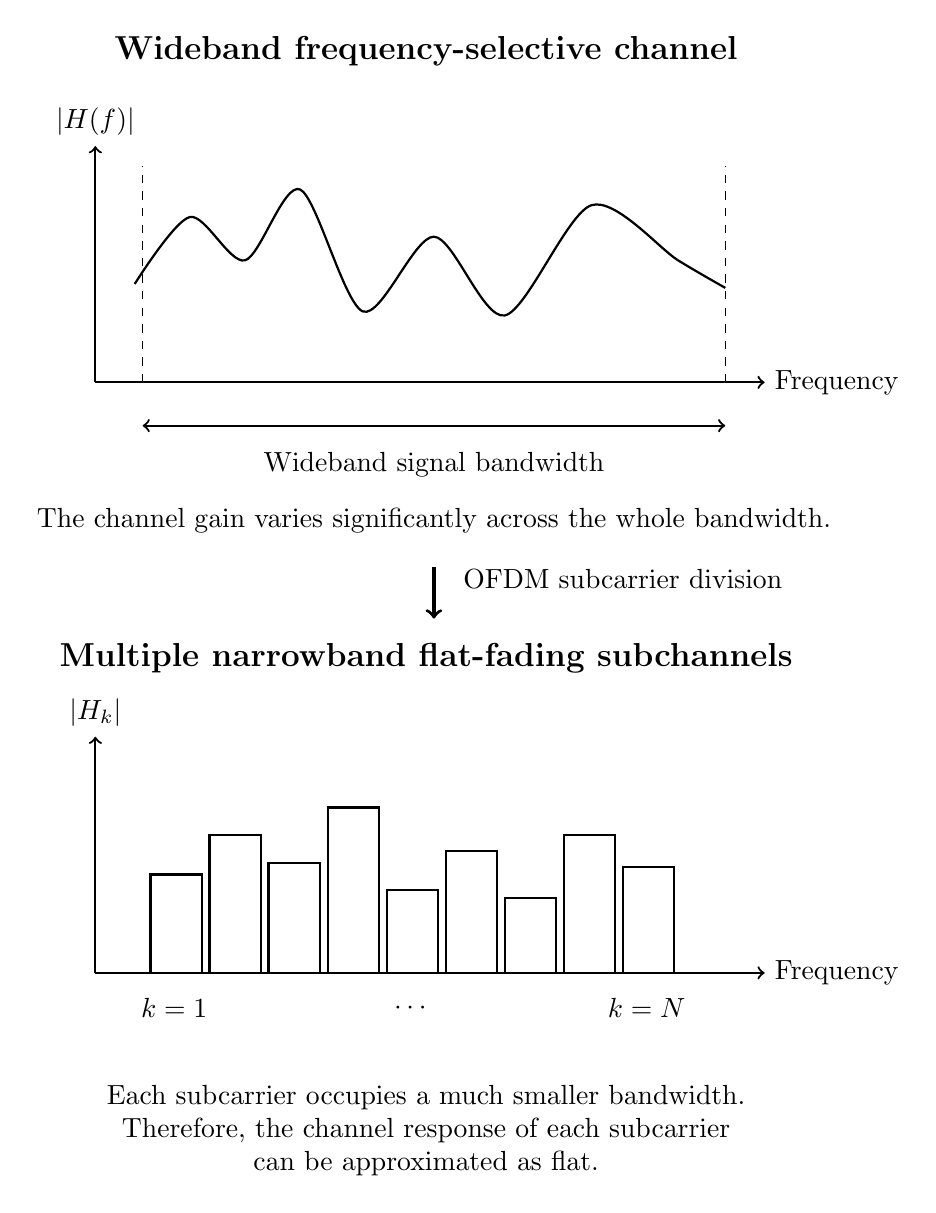
\begin{tikzpicture}[
        every node/.style={font=\normalsize},
        axis/.style={->, thick},
        thickline/.style={thick}
    ]

    % =====================================================
    % Top: Wideband frequency-selective channel
    % =====================================================
    \node[font=\bfseries\large] at (4.2,4.2)
    {Wideband frequency-selective channel};

    \draw[axis] (0,0) -- (8.5,0) node[right] {Frequency};
    \draw[axis] (0,0) -- (0,3.0) node[above] {$|H(f)|$};

    % Frequency-selective response
    \draw[thickline]
        plot[smooth] coordinates {
        (0.5,1.25)
        (1.2,2.10)
        (1.9,1.55)
        (2.6,2.45)
        (3.4,0.90)
        (4.3,1.85)
        (5.2,0.85)
        (6.3,2.25)
        (7.4,1.55)
        (8.0,1.20)
        };

    % Bandwidth marks
    \draw[dashed] (0.6,0) -- (0.6,2.75);
    \draw[dashed] (8.0,0) -- (8.0,2.75);

    \draw[<->, thick] (0.6,-0.55) -- (8.0,-0.55);
    \node at (4.3,-1.05) {Wideband signal bandwidth};

    % Explanation label
    \node[align=center] at (4.3,-1.75)
    {The channel gain varies significantly across the whole bandwidth.};

    % =====================================================
    % Down arrow
    % =====================================================
    \draw[->, very thick] (4.3,-2.35) -- (4.3,-3.0);
    \node[right] at (4.55,-2.5) {OFDM subcarrier division};

    % =====================================================
    % Bottom: Narrowband subchannels
    % =====================================================
    \begin{scope}[yshift=-7.5cm]

    \node[font=\bfseries\large] at (4.2,4.0)
    {Multiple narrowband flat-fading subchannels};

    \draw[axis] (0,0) -- (8.5,0) node[right] {Frequency};
    \draw[axis] (0,0) -- (0,3.0) node[above] {$|H_k|$};

    % Draw narrow flat subchannels
    \draw[thick] (0.7,0) rectangle (1.35,1.25);
    \draw[thick] (1.45,0) rectangle (2.10,1.75);
    \draw[thick] (2.20,0) rectangle (2.85,1.40);
    \draw[thick] (2.95,0) rectangle (3.60,2.10);
    \draw[thick] (3.70,0) rectangle (4.35,1.05);
    \draw[thick] (4.45,0) rectangle (5.10,1.55);
    \draw[thick] (5.20,0) rectangle (5.85,0.95);
    \draw[thick] (5.95,0) rectangle (6.60,1.75);
    \draw[thick] (6.70,0) rectangle (7.35,1.35);

    % Labels
    \node at (1.0,-0.45) {$k=1$};
    \node at (4.0,-0.45) {$\cdots$};
    \node at (7.0,-0.45) {$k=N$};

    \node[align=center] at (4.2,-2)
    {Each subcarrier occupies a much smaller bandwidth.\\
    Therefore, the channel response of each subcarrier\\
    can be approximated as flat.};

    \end{scope}

    \end{tikzpicture}
    }

    \caption{Conversion of a frequency-selective wideband channel into multiple narrowband flat-fading subchannels in OFDM.}
    \label{fig:ofdm_parallel_subchannels}
\end{figure}


OFDM also provides high spectral efficiency due to the orthogonality among subcarriers. Unlike conventional frequency division multiplexing, which requires guard bands between adjacent carriers, OFDM allows subcarrier spectra to overlap while still avoiding mutual interference under ideal conditions. This property makes OFDM particularly suitable for bandwidth-limited wireless communication systems.

The main advantages of OFDM are summarized in Table~\ref{tab:ofdm_advantages}.

\begin{table}[H]
\centering
\caption{Main advantages of OFDM systems.}
\label{tab:ofdm_advantages}

\begin{tabular}{|p{4cm}|p{8cm}|}
\hline
\textbf{Advantage} &
\textbf{Description} \\
\hline

High spectral efficiency &
Overlapping orthogonal subcarriers reduce the need for guard bands. \\
\hline

Robustness to multipath &
Longer symbol duration and cyclic prefix reduce the effect of delay spread. \\
\hline

Simple equalization &
Frequency-selective channels are transformed into parallel flat-fading subchannels. \\
\hline

FFT-based implementation &
IFFT and FFT operations enable efficient digital implementation. \\
\hline

Flexible resource allocation &
Subcarriers can be assigned adaptively according to channel conditions and user requirements. \\
\hline

\end{tabular}

\end{table}

Despite these advantages, OFDM relies heavily on the preservation of subcarrier orthogonality. This requirement becomes difficult to satisfy in rapidly time-varying wireless channels, especially when the receiver operates under high mobility. The limitations of OFDM under such conditions are discussed in the following subsection.

\subsubsection{Limitations of OFDM in High-Mobility Environments}

Although OFDM is highly effective in combating frequency-selective fading, its performance can degrade significantly in high-mobility environments. The main reason is that OFDM assumes the wireless channel remains approximately constant during one OFDM symbol duration. When this assumption is violated, the orthogonality among subcarriers is destroyed.

In high-mobility scenarios, relative motion between the transmitter, receiver, and scatterers introduces Doppler shifts. These Doppler shifts cause the channel response to vary within an OFDM symbol interval. Consequently, the received signal is no longer affected only by the channel gain on its own subcarrier, but also by leakage from neighboring subcarriers. This phenomenon is known as inter-carrier interference (ICI).

Under ideal conditions, the received signal on the \(k\)-th subcarrier is represented by

\begin{equation}
Y[k]=H[k]X[k]+W[k].
\end{equation}

However, in the presence of Doppler-induced channel variation, the received signal becomes

\begin{equation}
Y[k]=H[k]X[k]+\sum_{\substack{m=0 \\ m\neq k}}^{N-1} I[k,m]X[m]+W[k],
\end{equation}

where \(I[k,m]\) represents the interference contribution from the \(m\)-th subcarrier to the \(k\)-th subcarrier. The second term in the equation represents inter-carrier interference caused by the loss of orthogonality.

\begin{figure}[H]
    \centering
    
\includegraphics[width=1\textwidth]{Images/Chapter2/ici.png}
    \caption[Inter-carrier interference in OFDM caused by Doppler-induced loss of subcarrier orthogonality.]{Inter-carrier interference in OFDM caused by Doppler-induced loss of subcarrier orthogonality~\protect\cite{Hong2019OTFSTutorial}.}
    \label{fig:ofdm_ici}
\end{figure}

As illustrated in Fig.~\ref{fig:ofdm_ici}, Doppler shifts disturb the frequency-domain alignment of OFDM subcarriers. The null points of one subcarrier no longer coincide with the peaks of other subcarriers, causing interference among subcarriers. This effect becomes more severe as the Doppler spread increases.

Another limitation of OFDM is that the performance of the system is strongly affected by the weakest subcarriers. In a frequency-selective fading channel, some subcarriers may experience deep fading while others maintain strong channel gains. Although coding and interleaving can mitigate this problem to some extent, the overall reliability of the system may still be limited by poorly conditioned subchannels.

Furthermore, the one-tap equalization structure of OFDM is only effective when the channel matrix remains nearly diagonal in the frequency domain. In high-Doppler conditions, the channel matrix loses this diagonal structure due to ICI. Equalization therefore becomes more complex, and the simplicity that makes OFDM attractive is partially lost.

\begin{table}[H]
\centering
\caption{Main limitations of OFDM in high-mobility environments.}
\label{tab:ofdm_limitations}

\begin{tabular}{|p{4cm}|p{8cm}|}
\hline
\textbf{Limitation} &
\textbf{Impact} \\
\hline

Sensitivity to Doppler spread &
Doppler shifts destroy subcarrier orthogonality and introduce ICI. \\
\hline

Channel time variation &
The channel may change within one OFDM symbol, violating the quasi-static channel assumption. \\
\hline

Deep fading on subcarriers &
Some subcarriers may experience severe attenuation, reducing reliability. \\
\hline

Increased equalization complexity &
The channel matrix is no longer diagonal under severe Doppler conditions. \\
\hline

Performance degradation in high mobility &
BER increases significantly in vehicular, high-speed railway, UAV, and satellite communication scenarios. \\
\hline

\end{tabular}

\end{table}

These limitations motivate the search for alternative waveform designs that can better handle doubly selective channels. Instead of representing information symbols only in the time-frequency domain, OTFS modulation introduces a delay-Doppler domain representation where the channel can be described more compactly and more stably under high mobility. Before introducing OTFS in detail, the next section reviews the delay-Doppler domain representation of wireless channels.


\subsection{Delay-Doppler Domain Representation}

The analysis of high-mobility wireless channels requires a signal representation that can describe both multipath propagation and Doppler effects. Conventional multicarrier systems such as OFDM usually describe signal transmission in the time-frequency domain. This representation is convenient for practical implementation, because data symbols can be arranged over time slots and frequency subcarriers.

However, in high-mobility environments, the wireless channel may vary rapidly over time due to Doppler effects. As a result, the time-frequency channel coefficients can change significantly from one resource element to another. This makes channel estimation and equalization more difficult. For this reason, the delay-Doppler domain is introduced as an alternative representation that is more closely related to the physical propagation paths of the wireless channel.

The delay-Doppler representation is an important foundation for OTFS modulation. Instead of describing the channel only by its variations over time and frequency, this representation describes the channel using propagation delay and Doppler shift. These two quantities correspond directly to multipath propagation and relative motion, respectively.

\subsubsection{Time-Frequency Domain}

The time-frequency domain is widely used in modern wireless communication systems, especially in OFDM-based transmission. In this representation, the available transmission resources are divided into time slots and frequency subcarriers. Each information symbol is placed on a specific time-frequency resource element.

The time axis represents consecutive OFDM symbols or time slots, while the frequency axis represents the orthogonal subcarriers. Therefore, each cell in the time-frequency grid corresponds to one symbol position in both time and frequency. This structure is suitable for OFDM because one OFDM symbol occupies a time interval and contains multiple subcarriers in the frequency domain.

\begin{figure}[H]
\centering
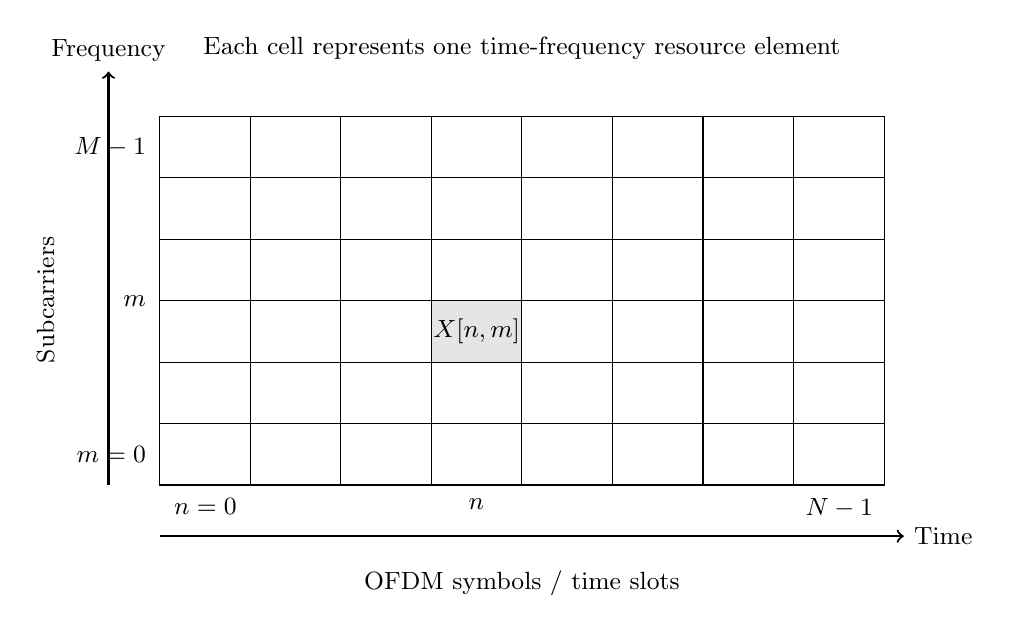
\begin{tikzpicture}[every node/.style={font=\small}]

    % Grid parameters
    \def\cw{1.15}
    \def\ch{0.78}

    % Draw grid
    \foreach \i in {0,...,7} {
        \foreach \j in {0,...,5} {
            \draw (\i*\cw,\j*\ch) rectangle ++(\cw,\ch);
        }
    }

    % Highlight one resource element
    \filldraw[fill=gray!20, draw=black] (3*\cw,2*\ch) rectangle ++(\cw,\ch);
    \node at (3*\cw+0.5*\cw,2*\ch+0.5*\ch) {$X[n,m]$};

    % Axes
    \draw[->, thick] (-0.65,0) -- (-0.65,5.25) node[above] {Frequency};
    \draw[->, thick] (0,-0.65) -- (9.45,-0.65) node[right] {Time};

    % Axis descriptors
    \node[rotate=90] at (-1.45,2.35) {Subcarriers};
    \node at (4.6,-1.25) {OFDM symbols / time slots};

    % Labels on vertical axis
    \node[left] at (-0.05,0.39) {$m=0$};
    \node[left] at (-0.05,2.34) {$m$};
    \node[left] at (-0.05,4.29) {$M-1$};

    % Labels on horizontal axis
    \node[below] at (0.58,-0.05) {$n=0$};
    \node[below] at (4.02,-0.05) {$n$};
    \node[below] at (8.63,-0.05) {$N-1$};

    % Top explanation
    \node at (4.6,5.55) {Each cell represents one time-frequency resource element};

\end{tikzpicture}
\caption{Time-frequency grid representation used in multicarrier transmission systems.}
\label{fig:time_frequency_grid}

\end{figure}

Figure~\ref{fig:time_frequency_grid} illustrates the time-frequency grid structure. In OFDM, data symbols are directly assigned to this grid. The receiver then processes the received signal in the frequency domain using FFT-based operations. This approach is effective when the channel is approximately constant during one OFDM symbol interval.

Nevertheless, the time-frequency representation becomes less stable in high-mobility environments. When the transmitter, receiver, or surrounding scatterers move rapidly, the channel changes during transmission. Consequently, the channel response in the time-frequency domain may fluctuate quickly across both time and frequency. This effect can destroy the orthogonality among OFDM subcarriers and introduce inter-carrier interference.

Although the time-frequency domain is convenient for waveform generation and practical implementation, it does not always provide the most compact description of doubly selective channels. This motivates the use of the delay-Doppler domain.

\subsubsection{Delay-Doppler Representation}

The delay-Doppler domain describes the wireless channel using two physical parameters: propagation delay and Doppler shift. The delay dimension is associated with multipath propagation. Different reflected paths travel different distances before reaching the receiver, so they arrive at different times. The Doppler dimension is associated with relative motion. When the transmitter, receiver, or scatterers are moving, each path may experience a frequency shift.

In this representation, each dominant propagation path can be described by three main parameters: its path gain, its delay, and its Doppler shift. Therefore, instead of viewing the channel as a rapidly changing surface over time and frequency, the delay-Doppler domain views it as a collection of physical propagation paths.

A simple delay-Doppler channel model can be expressed as

\begin{equation}
h(\tau,\nu)
=
\sum_{i=1}^{P}
h_i
\delta(\tau-\tau_i)
\delta(\nu-\nu_i),
\end{equation}

where \(P\) denotes the number of dominant propagation paths. The parameter \(h_i\) represents the complex gain of the \(i\)-th path, while \(\tau_i\) and \(\nu_i\) denote its delay and Doppler shift, respectively.

This equation means that the channel can be interpreted as the sum of several dominant propagation components. Each component appears at a certain delay and a certain Doppler shift. In many practical wireless channels, only a limited number of propagation paths carry significant energy. Therefore, the delay-Doppler channel representation is often sparse.

\begin{figure}[H]
\centering
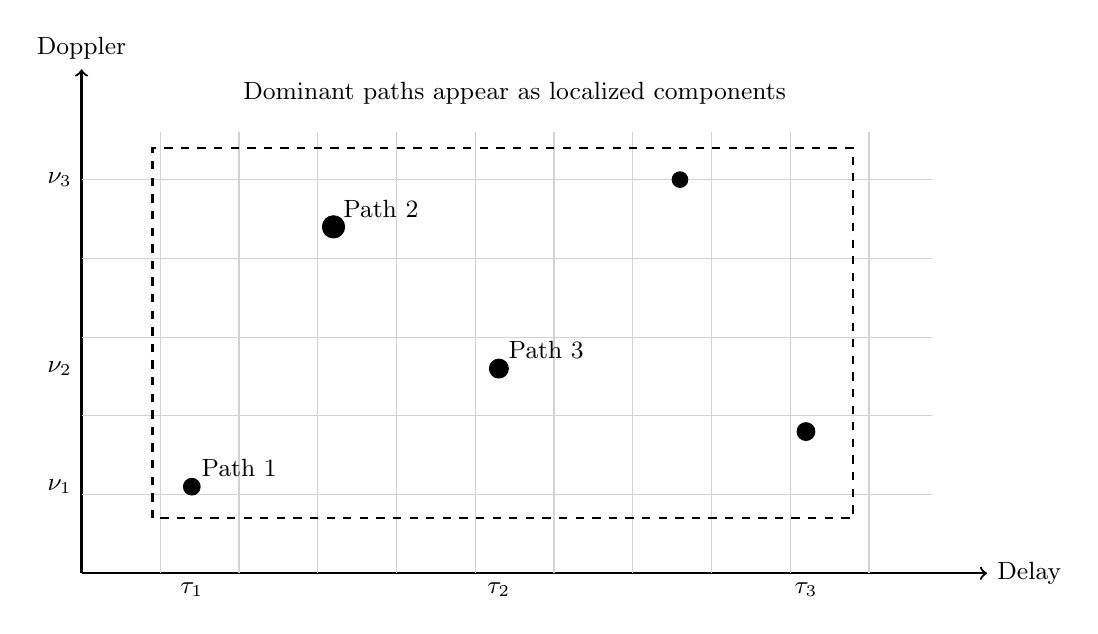
\begin{tikzpicture}[
every node/.style={font=\small},
axis/.style={->, thick},
gridline/.style={gray!35, thin}
]

    % Axes
    \draw[axis] (0,0) -- (11.5,0) node[right] {Delay};
    \draw[axis] (0,0) -- (0,6.4) node[above] {Doppler};

    % Grid
    \foreach \x in {1,2,...,10} {
        \draw[gridline] (\x,0) -- (\x,5.6);
    }

    \foreach \y in {1,2,3,4,5} {
        \draw[gridline] (0,\y) -- (10.8,\y);
    }

    % Sparse dominant paths
    \filldraw[black] (1.4,1.1) circle (3.0pt);
    \filldraw[black] (3.2,4.4) circle (4.0pt);
    \filldraw[black] (5.3,2.6) circle (3.4pt);
    \filldraw[black] (7.6,5.0) circle (2.8pt);
    \filldraw[black] (9.2,1.8) circle (3.2pt);

    % Path labels
    \node[above right] at (1.4,1.1) {Path 1};
    \node[above right] at (3.2,4.4) {Path 2};
    \node[above right] at (5.3,2.6) {Path 3};

    % Sparse support region
    \draw[dashed, thick] (0.9,0.7) rectangle (9.8,5.4);

    % Axis tick labels
    \node[below] at (1.4,0) {$\tau_1$};
    \node[below] at (5.3,0) {$\tau_2$};
    \node[below] at (9.2,0) {$\tau_3$};

    \node[left] at (0,1.1) {$\nu_1$};
    \node[left] at (0,2.6) {$\nu_2$};
    \node[left] at (0,5.0) {$\nu_3$};

    % Annotation
    \node[align=center] at (5.5,6.1)
    {Dominant paths appear as localized components};

\end{tikzpicture}
\caption{Sparse representation of dominant multipath components in the delay-Doppler domain.}
\label{fig:delay_doppler_channel}

\end{figure}

As illustrated in Fig.~\ref{fig:delay_doppler_channel}, each significant propagation path appears as a localized component in the delay-Doppler plane. The horizontal coordinate represents the propagation delay, while the vertical coordinate represents the Doppler shift. Since the number of dominant paths is usually limited, the channel energy is concentrated around several points or small regions.

This sparse representation is useful in high-mobility communications. In the time-frequency domain, the channel coefficients may vary rapidly due to Doppler effects. In the delay-Doppler domain, however, the physical path parameters usually vary more slowly. This makes the delay-Doppler domain more suitable for describing doubly selective wireless channels.

Compared with the time-frequency domain, the delay-Doppler domain provides a more compact and physically meaningful description of the wireless channel. This is one of the main motivations for OTFS modulation.

\subsubsection{Relationship Between Signal Domains}

The time-frequency and delay-Doppler domains are not independent representations. They describe the same wireless communication system from different viewpoints. The time-frequency domain is convenient for practical waveform generation, while the delay-Doppler domain is more suitable for describing physical channel behavior in high-mobility scenarios.

In conventional OFDM systems, information symbols are placed directly on the time-frequency grid. Each symbol is associated with a particular OFDM symbol index and subcarrier index. In contrast, OTFS places information symbols on the delay-Doppler grid first. These symbols are then transformed into the time-frequency grid before transmission.

This transformation is performed by the inverse symplectic finite Fourier transform (ISFFT). At the receiver, after the signal has passed through the wireless channel and has been processed in the time-frequency domain, the symplectic finite Fourier transform (SFFT) is used to transform the received samples back into the delay-Doppler domain.

Instead of presenting the full mathematical expressions of these transforms here, the main idea can be understood as follows. The ISFFT spreads each delay-Doppler symbol over the time-frequency plane before transmission. After reception, the SFFT collects the received time-frequency information back into the delay-Doppler domain. Therefore, the two transforms form a bridge between the physical delay-Doppler representation and the practical time-frequency transmission structure.

\begin{figure}[H]
\centering
\resizebox{0.96\linewidth}{!}{%
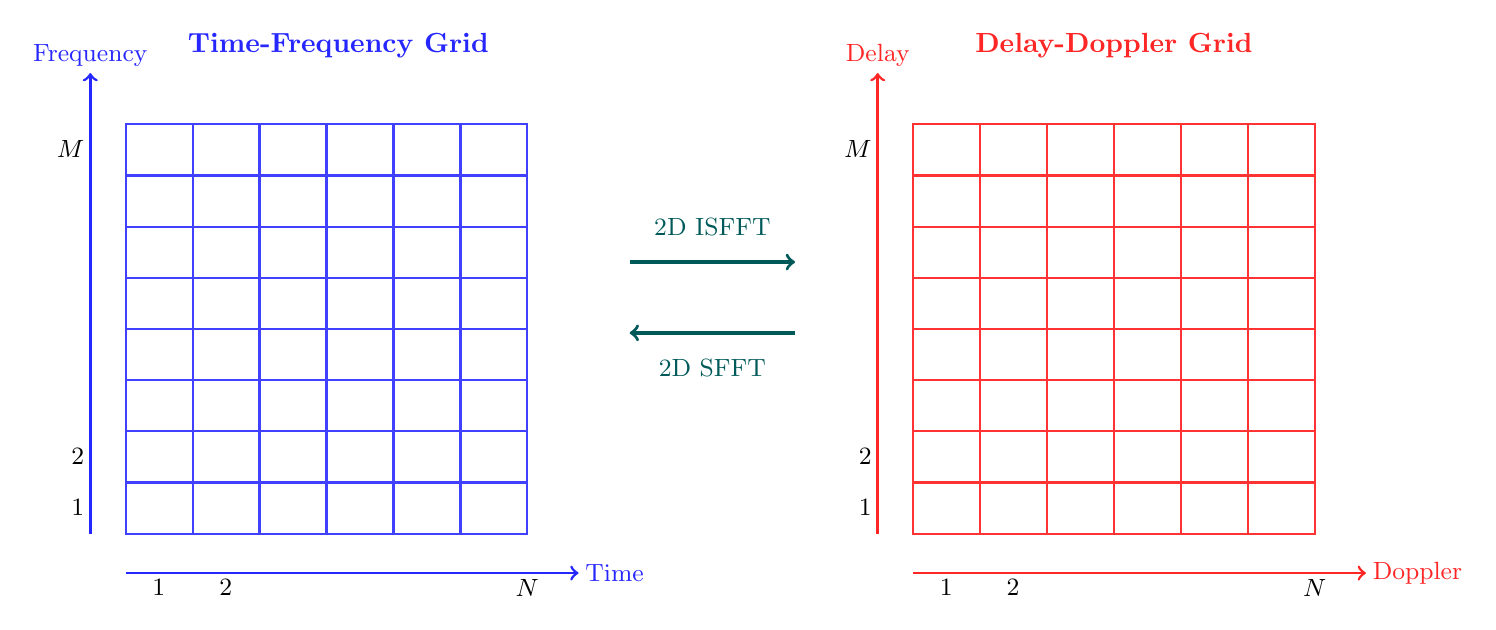
\begin{tikzpicture}[every node/.style={font=\small, inner sep=2pt}]

    % Parameters
    \def\cw{0.85}
    \def\ch{0.65}

    % =====================================================
    % Left grid: Time-Frequency
    % =====================================================
    \begin{scope}[shift={(0,0)}]

        \foreach \i in {0,...,5} {
            \foreach \j in {0,...,7} {
                \draw[blue!75, line width=0.8pt] (\i*\cw,\j*\ch) rectangle ++(\cw,\ch);
            }
        }

        \draw[->, blue!85, line width=1pt] (-0.45,0) -- (-0.45,5.85) node[above] {Frequency};
        \draw[->, blue!85, line width=1pt] (0,-0.5) -- (5.75,-0.5) node[right] {Time};

        \node[below] at (0.42,-0.5) {$1$};
        \node[below] at (1.27,-0.5) {$2$};
        \node[below] at (5.10,-0.5) {$N$};

        \node[left] at (-0.45,0.33) {$1$};
        \node[left] at (-0.45,0.98) {$2$};
        \node[left] at (-0.45,4.88) {$M$};

        \node[blue!85, font=\bfseries] at (2.7,6.2) {Time-Frequency Grid};

    \end{scope}

    % =====================================================
    % Middle arrows
    % =====================================================
    \draw[->, teal!70!black, line width=1.2pt] (6.4,3.45) -- (8.5,3.45);
    \node[teal!70!black] at (7.45,3.9) {2D ISFFT};

    \draw[->, teal!70!black, line width=1.2pt] (8.5,2.55) -- (6.4,2.55);
    \node[teal!70!black] at (7.45,2.1) {2D SFFT};

    % =====================================================
    % Right grid: Delay-Doppler
    % =====================================================
    \begin{scope}[shift={(10.0,0)}]

        \foreach \i in {0,...,5} {
            \foreach \j in {0,...,7} {
                \draw[red!80, line width=0.8pt] (\i*\cw,\j*\ch) rectangle ++(\cw,\ch);
            }
        }

        \draw[->, red!85, line width=1pt] (-0.45,0) -- (-0.45,5.85) node[above] {Delay};
        \draw[->, red!85, line width=1pt] (0,-0.5) -- (5.75,-0.5) node[right] {Doppler};

        \node[below] at (0.42,-0.5) {$1$};
        \node[below] at (1.27,-0.5) {$2$};
        \node[below] at (5.10,-0.5) {$N$};

        \node[left] at (-0.45,0.33) {$1$};
        \node[left] at (-0.45,0.98) {$2$};
        \node[left] at (-0.45,4.88) {$M$};

        \node[red!85, font=\bfseries] at (2.55,6.2) {Delay-Doppler Grid};

    \end{scope}

\end{tikzpicture}
}
\caption{Relationship between time-frequency and delay-Doppler signal domains.}
\label{fig:tf_dd_relationship}

\end{figure}

As illustrated in Fig.~\ref{fig:tf_dd_relationship}, the delay-Doppler grid and the time-frequency grid are connected through two-dimensional transforms. The delay-Doppler grid is useful for symbol placement and channel interpretation, while the time-frequency grid is suitable for practical transmission using multicarrier waveforms.

This relationship is particularly important for OTFS. OTFS does not completely discard the time-frequency domain. Instead, it uses the delay-Doppler domain for data representation and then maps the symbols into the time-frequency domain for transmission. In this way, OTFS can remain compatible with multicarrier transmission principles while exploiting the physical delay and Doppler characteristics of high-mobility wireless channels.

Table~\ref{tab:signal_domain_relationship} summarizes the main differences between the two domains.

\begin{table}[H]
\centering
\caption{Comparison between time-frequency and delay-Doppler signal domains.}
\label{tab:signal_domain_relationship}

\renewcommand{\arraystretch}{1.35}
\begin{tabularx}{\textwidth}{|
>{\RaggedRight\arraybackslash}p{3.0cm}|
>{\RaggedRight\arraybackslash}X|
>{\RaggedRight\arraybackslash}X|}
\hline
\textbf{Aspect} &
\textbf{Time-Frequency Domain} &
\textbf{Delay-Doppler Domain} \\
\hline

Signal coordinates &
Time and frequency indices &
Delay and Doppler indices \\
\hline

Typical use &
OFDM-based transmission &
OTFS-based transmission \\
\hline

Channel description &
Channel variation over time and frequency &
Physical paths with delay and Doppler shift \\
\hline

High-mobility behavior &
Rapidly varying channel coefficients &
Sparse and more stable path representation \\
\hline

Main transform &
FFT/IFFT operations &
SFFT/ISFFT operations \\
\hline

\end{tabularx}
\end{table}

Therefore, the delay-Doppler domain does not replace the time-frequency domain in practical implementation. Instead, it complements it. The time-frequency domain remains convenient for waveform generation and compatibility with OFDM architectures, while the delay-Doppler domain provides a more suitable representation for data placement and channel interpretation under high-mobility conditions. This idea forms the foundation of OTFS modulation, which is discussed in detail in Chapter 3.


% ~5 pages
\subsection{Index Modulation Fundamentals}

Index Modulation (IM) is a transmission concept in which information is conveyed not only through conventional modulation symbols but also through the indices of selected communication resources. These resources may correspond to subcarriers, antennas, time slots, spreading codes, or delay-Doppler resource elements depending on the considered system architecture. In this thesis, IM is introduced as a fundamental technique that later motivates the development of OTFS with Index Modulation.

Unlike conventional modulation schemes, where all information bits are mapped only onto constellation symbols, IM divides the information-carrying mechanism into two parts. A portion of the input bits determines the active resource indices, while the remaining bits are mapped onto conventional modulation symbols. This additional index dimension provides a flexible way to improve spectral efficiency and system design without necessarily increasing the modulation order.

\subsubsection{Principle of Index Modulation}

The basic principle of Index Modulation is to activate only a subset of available transmission resources during each transmission interval. The specific activation pattern itself carries information. For example, if a transmission block contains \(n\) available resource elements and only \(k\) of them are activated, the number of possible activation patterns is given by

\begin{equation}
N_{\mathrm{pattern}} = \binom{n}{k}.
\end{equation}

The number of bits that can be conveyed by the index pattern is therefore

\begin{equation}
p_1 = \left\lfloor \log_2 \binom{n}{k} \right\rfloor.
\end{equation}

In addition to these index bits, each active resource element transmits a conventional modulation symbol selected from an \(M_{\mathrm{mod}}\)-ary constellation. If \(k\) resource elements are active, the number of bits conveyed by the modulation symbols is

\begin{equation}
p_2 = k \log_2 M_{\mathrm{mod}}.
\end{equation}

Thus, the total number of transmitted bits per block can be written as

\begin{equation}
p = p_1 + p_2
=
\left\lfloor \log_2 \binom{n}{k} \right\rfloor
+
k \log_2 M_{\mathrm{mod}}.
\end{equation}

This formulation shows that IM conveys information through both the selected indices and the symbols transmitted on the active positions. The inactive positions are usually assigned zero values and do not transmit modulation symbols.

\begin{figure}[H]
\centering

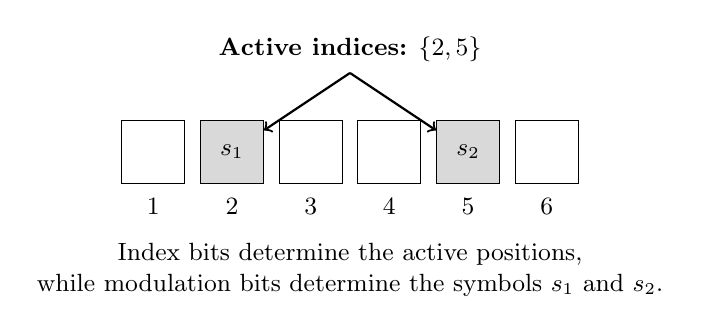
\begin{tikzpicture}[
    every node/.style={font=\small},
    active/.style={draw, fill=gray!30, minimum width=0.8cm, minimum height=0.8cm},
    inactive/.style={draw, minimum width=0.8cm, minimum height=0.8cm},
    arrow/.style={->, thick}
]

\node[align=center] at (2.5,1.3)
{\textbf{Active indices:} $\{2,5\}$};

\node[inactive] (r1) at (0,0) {};
\node[active]   (r2) at (1,0) {$s_1$};
\node[inactive] (r3) at (2,0) {};
\node[inactive] (r4) at (3,0) {};
\node[active]   (r5) at (4,0) {$s_2$};
\node[inactive] (r6) at (5,0) {};

\node at (0,-0.7) {\small 1};
\node at (1,-0.7) {\small 2};
\node at (2,-0.7) {\small 3};
\node at (3,-0.7) {\small 4};
\node at (4,-0.7) {\small 5};
\node at (5,-0.7) {\small 6};

\draw[arrow] (2.5,1.0) -- (r2);
\draw[arrow] (2.5,1.0) -- (r5);

\node[align=center] at (2.5,-1.5)
{Index bits determine the active positions,\\
while modulation bits determine the symbols $s_1$ and $s_2$.};

\end{tikzpicture}

\caption{Basic principle of index modulation using active resource elements.}
\label{fig:index_modulation_principle}
\end{figure}

As shown in Fig.~\ref{fig:index_modulation_principle}, only selected resource elements are activated in an IM-based transmission block. The receiver detects both the active indices and the transmitted constellation symbols in order to recover the original information bits.

\subsubsection{OFDM-IM Systems}

One of the most widely studied applications of Index Modulation is OFDM with Index Modulation (OFDM-IM). In conventional OFDM, all subcarriers are generally used to transmit constellation symbols. In OFDM-IM, however, only a subset of subcarriers within each subblock is activated, and the indices of these active subcarriers are used to convey additional information bits.

For an OFDM-IM subblock with \(n\) subcarriers, \(k\) active subcarriers, and \(M_{\mathrm{mod}}\)-ary modulation, the total number of transmitted bits per subblock is given by

\begin{equation}
p_{\mathrm{OFDM\text{-}IM}}
=
\left\lfloor \log_2 \binom{n}{k} \right\rfloor
+
k \log_2 M_{\mathrm{mod}}.
\end{equation}

The first term corresponds to the index bits, while the second term corresponds to the conventional modulation bits carried by the active subcarriers. Therefore, OFDM-IM can be viewed as an extension of OFDM in which subcarrier activation patterns introduce an additional information-carrying dimension.

\begin{figure}[H]
\centering

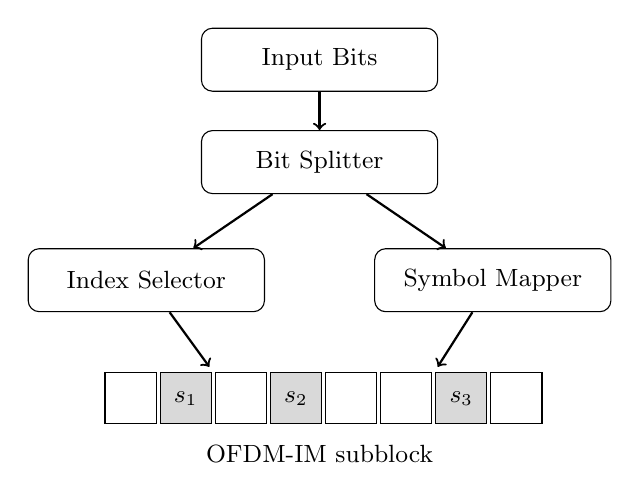
\begin{tikzpicture}[
    every node/.style={font=\small},
    block/.style={
        draw,
        rounded corners,
        minimum width=3.0cm,
        minimum height=0.8cm,
        align=center
    },
    arrow/.style={->, thick},
    active/.style={draw, fill=gray!30, minimum width=0.65cm, minimum height=0.65cm},
    inactive/.style={draw, minimum width=0.65cm, minimum height=0.65cm}
]

\node[block] (bits) at (0,0) {Input Bits};
\node[block] (split) at (0,-1.3) {Bit Splitter};
\node[block] (index) at (-2.2,-2.8) {Index Selector};
\node[block] (mapper) at (2.2,-2.8) {Symbol Mapper};

\draw[arrow] (bits) -- (split);
\draw[arrow] (split) -- (index);
\draw[arrow] (split) -- (mapper);

\node[inactive] (s1) at (-2.4,-4.3) {};
\node[active]   (s2) at (-1.7,-4.3) {$s_1$};
\node[inactive] (s3) at (-1.0,-4.3) {};
\node[active]   (s4) at (-0.3,-4.3) {$s_2$};
\node[inactive] (s5) at (0.4,-4.3) {};
\node[inactive] (s6) at (1.1,-4.3) {};
\node[active]   (s7) at (1.8,-4.3) {$s_3$};
\node[inactive] (s8) at (2.5,-4.3) {};

\node at (0,-5.0) {OFDM-IM subblock};

\draw[arrow] (index) -- (-1.4,-3.9);
\draw[arrow] (mapper) -- (1.5,-3.9);

\end{tikzpicture}

\caption{Conceptual structure of an OFDM-IM subblock.}
\label{fig:ofdm_im_subblock}
\end{figure}

The OFDM-IM concept provides a useful foundation for understanding more advanced IM-based systems. Since the present thesis focuses on OTFS-IM, the detailed mathematical design of OFDM-IM is not discussed extensively in this chapter. Instead, OFDM-IM is introduced as a representative example showing how index patterns can be exploited for information transmission.

\subsubsection{Advantages and Challenges of IM}

Index Modulation offers several attractive advantages for wireless communication systems. First, it provides an additional mechanism for conveying information without relying solely on constellation symbols. This can improve spectral efficiency or allow lower modulation orders to be used for a given transmission rate.

Second, IM offers flexibility in resource allocation. By changing the number of active resources, modulation order, and index mapping strategy, the system can be adapted to different performance requirements. For example, increasing the number of active resources may improve data rate, while reducing the number of active resources may reduce transmit energy and interference.

Third, IM can improve error performance in certain channel conditions because inactive resource elements provide additional structure that may assist detection at the receiver. The sparsity introduced by index activation can also be beneficial for receiver design, especially in systems where the channel itself has a sparse structure.

However, Index Modulation also introduces several challenges. The receiver must detect both the active indices and the transmitted symbols, which may increase detection complexity compared with conventional modulation. Furthermore, incorrect detection of active indices can lead to multiple bit errors because both index bits and symbol bits may be affected.

Another challenge is the design of efficient index mapping tables. Since the number of available activation patterns \(\binom{n}{k}\) is not always a power of two, only a subset of all possible patterns may be used in practical systems. This may lead to unused patterns and requires careful mapping design.

The main advantages and challenges of Index Modulation are summarized in Table~\ref{tab:im_advantages_challenges}.

\begin{table}[H]
\centering
\caption{Advantages and challenges of Index Modulation.}
\label{tab:im_advantages_challenges}

\small
\setlength{\tabcolsep}{6pt}
\begin{tabularx}{0.95\textwidth}{|>{\RaggedRight\arraybackslash}p{0.31\textwidth}|>{\RaggedRight\arraybackslash}X|}
\hline
\textbf{Aspect} &
\textbf{Description} \\
\hline

Additional information dimension &
Information is transmitted through both constellation symbols and active indices. \\
\hline

Flexible system design &
The number of active resources and modulation order can be adjusted according to system requirements. \\
\hline

Potential energy efficiency &
Only selected resources are active in each transmission block. \\
\hline

Detection complexity &
The receiver must jointly detect active indices and transmitted symbols. \\
\hline

Index detection errors &
Incorrect index detection may cause multiple bit errors. \\
\hline

Mapping design &
Efficient mapping is required when the number of activation patterns is not a power of two. \\
\hline

\end{tabularx}

\end{table}

In the context of this thesis, Index Modulation is considered as a promising technique to enhance OTFS transmission. The detailed OTFS-IM system model, including index mapping in the delay-Doppler domain, transmitter structure, receiver detection, and performance evaluation, will be presented in Chapter 4.


\subsection{Chapter Summary}

This chapter presented the theoretical background required for the study of OTFS and OTFS-IM systems. The fundamental characteristics of wireless communication channels were first introduced, including channel impairments, channel classification, multipath propagation, delay spread, Doppler effects, and doubly selective fading channels.

The chapter then reviewed the principles of OFDM, including its transceiver structure, advantages, and limitations in high-mobility environments. Although OFDM provides high spectral efficiency and simple frequency-domain equalization, its performance degrades significantly when severe Doppler spread destroys subcarrier orthogonality and introduces inter-carrier interference.

The delay-Doppler domain representation was also discussed as an alternative way to characterize time-varying wireless channels. This representation describes wireless propagation in terms of delay and Doppler shifts, providing a more suitable foundation for understanding OTFS modulation. Finally, the basic concept of Index Modulation was introduced, including its principle, OFDM-IM structure, advantages, and challenges.

Overall, this chapter established the necessary theoretical foundation for the following chapters. Based on these concepts, Chapter 3 will present the principles and mathematical formulation of OTFS modulation in more detail.

\newpage

\newpage
